\documentclass[leqno]{article}
\usepackage[utf8]{inputenc}
\usepackage[T1]{fontenc}
\author{Colin Roberts}
\title{Math 160  Lecture Notes - SP 2018}
\usepackage[left=3cm,right=3cm,top=3cm,bottom=3cm]{geometry}
\usepackage{amssymb, amsmath ,cleveref ,thmtools, amsthm, mathtools,tikz-cd,color,xcolor}
\usepackage{enumerate}


\makeatletter
\def\thmhead@plain#1#2#3{%
  \thmname{#1}\thmnumber{\@ifnotempty{#1}{ }\@upn{#2}}%
  \thmnote{ {\the\thm@notefont#3}}}
\let\thmhead\thmhead@plain
\makeatother
\theoremstyle{definition}
\newtheorem{definition}{Definition}[section]
\newtheorem{remark}{Remark}[section]
\newtheorem{example}{Example}[section]
\newtheorem{question}{Question}[section]
\newtheorem{exercise}{Exercise}[section]

\theoremstyle{remark}
\newtheorem*{solution}{Solution}

\theoremstyle{theorem}
\newtheorem{theorem}{Theorem}[section]
\newtheorem{corollary}{Corollary}[section]
\newtheorem{proposition}{Proposition}[section]

\newcommand{\R}{\mathbb{R}}
\newcommand{\Q}{\mathbb{Q}}

\begin{document}
\titlepage
\tableofcontents
\pagebreak

\section{Introductory Discussion}
\subsection{Why Calculus?}
\begin{question}
What is calculus? What is the point of it? Why should we care?
\end{question}

\noindent \emph{Answer:} Calculus is the study of functions on a small (\emph{infinitesimal}) or \emph{local} scale.  We will care about knowing how a function changes as we vary the input, the rate of change of functions at a point, and how we can use this to model the world around us.  Calculus allows us to understand how the change in one quantity will relate to a change in another quantity.  It turns out that most basic physical phenomena can be fully explained with elementary calculus and many extremely complicated phenomena require adding a bit more structure onto the calculus we will learn here.

\begin{question}
What was the motivation for creating/discovering calculus?
\end{question}

\noindent \emph{Answer:} Though it's argued who truly created/discovered calculus, it's usually attributed to Isaac Newton who found that he needed calculus in his study of the motion of objects and forces.  Many of you have/will/are taking PH141-PH142.  These courses are by no means co/prerequisites for MATH160, but many of the nice analogies, questions, and motivation will come from topics also found in physics.

\noindent \textbf{Instructor Note:} I will prefer to allude to physics because of my background in physics.  For me, it helps to understand mathematics when I can also understand it physically.  If this helps you, great! If it doesn't, then please feel free to let me know if there is something I can change.

\subsection{Mathematical Terminology You Will See}

Mathematics has a drawback when you are first learning it in that many new symbols, definitions, theorems, and more will pop up.  It's helpful to have a bank of these ideas to keep coming back to in order to make sure things make sense.  We generally start with a \emph{definition}, which is exactly what it seems like; here we create a new term in our dictionary and describe what this term means.  

We then have \emph{lemmas,} \emph{theorems}, and \emph{corollaries}. A theorem is simply a logical statement that follows from definitions we have created.  Lemmas are just like theorems, yet they are generally not as important or they are used to prove more important theorems. Corollaries usually follow theorems as direct, yet important, immediate results.

The word \emph{arbitrarily} will be tossed around a lot.  The typical example would be the statement, ``We can let $\delta>0$ be arbitrarily small." Here we just mean that we can make $\delta$ as small as we need, but still greater than $0$, in which there is no smallest number. There are times we may want to say that we can choose an ``arbitrarily large" number.  Again, this just means we pick a number as large as we'd like, since there is no largest number.

The idea of a \emph{set} will also show up.  A set is just a collection of objects.  In our class we will generally be concerned with sets of real numbers. Next, which is critically important for us, is the notion of a \emph{function}.  A function is defined to act on a \emph{domain} (input set) and output a \textbf{single value} in the \emph{range} (output set) of the function. It is important to remember functions output only a single value for any input value, otherwise a function would not pass the vertical line test.

\subsubsection{Brief Mention of Logic}

Logic is not something that will be covered in this course.  However, it is an important idea to understand so that you can fully grasp all of the content we see.  The important ideas are the following.

In logic, you will generally deal with statements and their implications.  For example, if we consider a statement $P$, we can say that $P$ implies $Q$ and write $P\implies Q$.  All this means is that if the statement $P$ is true, then the statement $Q$ is also true since $P\implies Q$.  Furthermore, we could have that a statement $P$ is true if and only if $Q$ is true.  In this case, we write $P\iff Q$.  What this tells us is that $P$ being true means that $Q$ is also true, and that $Q$ being true means that $P$ is also true.  

\subsection{Mathematical Symbols You Will See}

Here is a list of symbols you will find in our class (if more come, I will update this list):

\begin{enumerate}[1.]
\item $\R$, The set of \emph{real numbers}.
\item $\in$, ``Is a member of." (i.e. $\sqrt{2}\in \R$ can be read as, ``The square root of 2 is a member of the real numbers."
\item $\neq$, \underline{Not} equal to.
\item $\approx$, ``Approximately equal to."
\item $\coloneqq$, We are defining something, i.e., $\frac{df}{dx}\coloneqq \lim_{h\to 0}\frac{f(x+h)-f(x)}{h}$.
\item $\implies$, "Implies."
\item $\iff$, "If and only if."
\item $\therefore~$, "Therefore."
\item $\infty$, Infinity.  \emph{Note: Infinity is \underline{not} a number!}
\item $\Delta$, A change. (i.e. $\Delta x$ represents a change in the variable $x$).
\item $\delta$, Usually a small but positive value that is correlated to the input variable. Commonly used for denoting the error (uncertainty) in experimental measurement as well, for the same reason.
\item $\epsilon$, Usually a small but positive value that is correlated to the output variable. Sometimes used for denoting the error error (uncertainty) in experimental measurement.
\item $(a,b)$, The \emph{open} interval of real numbers from $a$ to $b$ that does not include $a$ or $b$. \emph{Note: sometimes we will also use this to say the point in the plane with $x=a$ and $y=b$, so be careful! Context clues will tell you which is intended.}
\item $[a,b]$, The \emph{closed} interval of real numbers from $a$ to $b$ including $a$ and $b$.
\item $(a,b]$, The \emph{half-open} interval of real numbers from $a$ to $b$ not including $a$ but including $b$. Similar for $[a,b)$.
\item $\{a,b\}$, The set containing $a$ and $b$. Likely won't use this much, but remember that $\{$ $\}$ will denote a set as opposed to an interval.
\item $x_i$, We usually use subscripts to label certain quantities.  Here we would say ``$x$-sub-$i$".  Many times this will make more physical sense, like labeling $t_i$ or $t_1$ as the initial time.
\item $[a]$, The physical unit denoted by $a$. Also won't use this much, but remember that $[$ $]$ will tell us that what inside is to be thought of as a physical unit, i.e., $[m]$ would denote meters.
\end{enumerate}

\pagebreak


\section{Limits and Continuity, Lecture Notes: \S 2.1 - 1/17/2018}

Chapter 2 of our text is all about \emph{limits} of functions and \emph{continuous} functions. These are very important ideas in calculus and we will find that everything we do will be built off of these ideas.  Moreover, limits take the front seat as being how we can define continuous functions and more.  These notions are important, and its in one's best interest to make sure to nail these down early.

The main ideas are as follows: Sometimes functions aren't as ``nice" as we want them to be, and for example we may have an input to the function in which the function has no defined output. Take for example:
\[
f(x)=\frac{x^2-1}{x-1};
\]
at $x=1$ the function is not defined since we cannot divide by zero, but the function appears to get closer and closer to outputting 2 as $x$ gets closer and closer to 1. Check this for yourself if you don't believe me! This is because when $x\neq 1$, we have that
\[
f(x)=\frac{x^2-1}{x-1}=\frac{(x-1)(x+1)}{x-1}=x+1.
\]
We will get to the bottom of this in the following sections.

\subsection{Rates of Change and Tangents to Curves}

Many times it is helpful to imagine (or model) a function $f$ describes the position of a particle.  We would say that $f(t)$ would be the position of the particle at time $t$.  Assuming we don't have a completely boring example, then our particle would then be changing position as time changes.  

Since we know where the thing is at all times, we might begin to ask, ``Well how fast is it going at time $t$?" The solution here is not immediately obvious, or even necessarily possible, but what we can do is calculate the average speed of this particle from time $t_1$ to $t_2$, where $t_1$ and $t_2$ are arbitrary times in which we measured the particle position. This is to say that the times $t_1$ and $t_2$ are in the domain of the function $f$. 

\begin{definition}
The \emph{average speed} during an interval of time $[t_1,t_2]$ is the distance traveled over this interval divided by the time elapsed. If $s(t)$ is the distance traveled at time $t$, then 
\[
\frac{s(t_2)-s(t_1)}{t_2-t_1}=\frac{\Delta s}{\Delta t}
\]
is the average speed over the interval $[t_1,t_2]$.
\end{definition}

\begin{exercise}
Objects near Earth experience a gravitational acceleration of $9.8[m/s^2]$. Imagine an object perched high in the atmosphere that begins falling at $t=0$. We know that the distance traveled after $t$ seconds is given by $s(t)=\frac{9.8}{2}t^2[m]$. Find the average speed from $t=0$ to $t=15$. Finally, find the average speed from $t=10$ to $t=15$.
\end{exercise}
\vspace*{4cm}

\begin{definition}
The \emph{average rate of change of $y=f(x)$ with respect to $x$ over the interval $[x_1,x_2]$} is 
\[
\frac{\Delta y}{\Delta x}=\frac{f(x_2)-f(x_1)}{x_2-x_1}=\frac{f(x_1+h)-f(x_1)}{h} ~~~~ h\neq 0,
\]
where $h$ is just the distance $x_2$ is away from $x_1$.
\end{definition}

Now, what if we would like to use this average rate of change to approximate the function $f$ over the interval? It turns out that the average rate of change allows us to find a secant line between the two endpoints of our interval, and this secant line is a good linear approximation of the function between those endpoints.

\begin{definition}
A \emph{secant line} is a line joining two points of a curve (graph of a function). The average rate of change is the slope of the secant line.  The two points will generally be the endpoints of the interval we found the average rate of change over.
\end{definition}
\vspace*{4cm}

\noindent \textbf{Recall:} We have two important ways of writing the equation for a line:
\begin{enumerate}[1.]
\item Point-Slope form: $y-y_1=m(x-x_1)$,
\item Slope-Intercept form: $y=mx+b$.
\end{enumerate}
Keep these memorized as it will be important to know which is which.

\begin{exercise}
Using the function from our first exercise, $s(t)=\frac{9.8}{2}t^2$, find the equation of the secant line that approximates the function $s$ on the interval $[1,4]$.  Find both the point-slope and the slope-intercept form and graph the secant line and $s$.
\end{exercise}
\vspace*{4cm}

Now, we would next like to know the answer to our original question in how we could know how fast the object moves at each moment.  Yet, we're still stuck on how to do this.  Let's keep building more machinery.

\begin{definition}
A \emph{tangent line} to a curve at a point $P$ is a line that just touches the curve at $P$.
\end{definition}
\vspace*{4cm}

If we were to use the secant line equation, we will end up with nonsense. This is because we are considering just a single point, and not two distinct endpoints.  If we plug in just one point into the average rate of change equation we will find 
\[
\frac{f(x)-f(x)}{x-x}=\frac{0}{0}.
\]

This brings us to the idea of a limit.  If we have points $P$ and $Q$ on a curve, then as $Q$ moves towards $P$ we find that the secant line between $P$ and $Q$ approach the tangent line to the curve at the point $P$.
\vspace*{4cm}

If we go back to the average rate of change equation, we see things more clearly when we write it as
\[
\frac{\Delta y}{\Delta x}=\frac{f(x+h)-f(x)}{h}, ~~~ h\neq 0.
\]

\begin{question}
Here, what is happening to $h$ as $Q$ moves towards $P$?
\end{question}

\noindent \emph{Answer:} 
\vspace*{2cm}

\begin{exercise}~
\begin{enumerate}[(a)]
\item What is the slope of the tangent line for the curve $f(x)=x^2+1$ at $P=(-1,2)$? \emph{Hint: Use the average change equation with the $h$ above and plug in the $x$ and $y$ values for $P$ properly. You should end up with a number added with $h$, but $h$ will go to zero as we approach $P$.}
\item Find the equation of the tangent line in both point-slope and slope-intercept.  \emph{Tip: Use point-slope,  then find slope-intercept.}
\end{enumerate}
\end{exercise}
\vspace*{6cm}

We generally think of the tangent line of $f$ at a point $P$ as the \emph{instantaneous rate of change of $f$ at $P$}.  This is exactly what we were aiming to find. Say $f$ models the position of a particle, then the slope of the tangent line would tell use how fast the particle is moving at that time!

\subsection{Limit of a Function and Limit Laws, Lecture Notes \S 2.2 - 1/19/2018}

\noindent \textbf{Recall:} Remember how the function 
\[
f(x)=\frac{x^2-1}{x-1}
\]
behaves near $x=1$.  We can't plug in $x=1$ since we cannot divide by zero, but for all other values of $x$, we have
\[
f(x)=\frac{(x-1)(x+1)}{x-1}=x+1, ~~~ x\neq 1.
\]
Then if we draw the graph of this function, we see that $f$ looks like the line $y=x+1$ with the point $(1,2)$ removed.
\vspace*{4cm}

\begin{exercise}
Given the following $x$ values, compute $f(x)$.  
\begin{enumerate}[1.]
\item $x=0.9$, $f(x)=$
\item $x=0.99$, $f(x)=$
\item $x=0.999$, $f(x)=$
\item $x=1.1$, $f(x)=$
\item $x=1.01$, $f(x)=$
\item $x=1.001$, $f(x)=$
\end{enumerate}
\end{exercise}
So we see that as $x$ nears $1$, the function is approaching (gets arbitrarily close to) $2$. We then say that, ``$f$ approaches the \emph{limit} 2 as $x$ approaches 1 and write
\[
\lim_{x\to 1} f(x)=2.
\]
More generally, for a function $f$  that approaches the limit $L$ as $x$ approaches $c$ we have
\[
\lim_{x\to c} f(x) = L.
\]

\begin{example}
Consider the following 3 functions:
\begin{enumerate}[1.]
\item $f(x)=\frac{x^2-1}{x-1}$,
\item $g(x)=
\begin{cases}
\frac{x^2-1}{x-1}, & x\neq 1\\
1, & x=1
\end{cases}$
\item $h(x)=x+1$.
\end{enumerate}
Draw these functions below. 
\vspace*{4cm}

Notice that $\lim_{x\to 1} f(x) = 2$ even though $f$ isn't defined at $x=1$, $\lim_{x\to 1} g(x)=2$ even though $g(1)\neq 2$, and $\lim_{x\to 1} h(x)=2$ which is also the same as $h(1)$.
\end{example}

\begin{example}
These are two important functions to remember:
\begin{enumerate}[1.]
\item The \emph{identity function} $f(x)=x$.  We have for any value of $c$ that
\[
\lim_{x\to c}f(x)=\lim_{x\to c} x = c.
\]
\item The \emph{constant function} $f(x)=k$. We have for any value of $c$ that
\[
\lim_{x\to c}f(x)=\lim_{x\to c} k = k.
\]
\end{enumerate}
\end{example}

It's a good idea to get a visual understanding for limits.  For the functions you drew above, remember what the limits were and the picture that goes along with it.  We will now look at three more other cases.

\begin{exercise}
For the following three functions, draw the graphs and explain what the limit as $x$ approaches $0$ should be.
\begin{enumerate}[1.]
\item $U(x)=
\begin{cases}
0, & x<0\\
1, & x\geq 0.
\end{cases}$
\item $g(x)=
\begin{cases}
\frac{1}{x}, & x\neq 0\\
0, & x=0.
\end{cases}$
\item $f(x)=
\begin{cases}
0, & x\leq 0\\
\sin\frac{1}{x}, & x>0.
\end{cases}$
\end{enumerate}
\vspace*{6cm}
\end{exercise}

\subsubsection{Limit Laws}

The following theorem will allow us to have an easier time finding limits of more complicated functions.

\begin{theorem}[(Limit Laws)]
\label{theorem: limit_laws}
If $L, M, c$ and $k$ are real numbers and
\[
\lim_{x\to c} f(x)=L ~~~~ and ~~~~ \lim_{x\to c} g(x)=M, ~~~~ \textrm{then}
\]
\begin{enumerate}[1.]
\item Sum Rule: $\lim_{x\to c} (f(x)+g(x))=L+M$
\item Difference Rule: $\lim_{x\to c} (f(x)-g(x))=L-M$
\item Constant Multiple Rule: $\lim(k\cdot f(x))=k\cdot L$
\item Product Rule: $\lim_{x\to c}(f(x)\cdot g(x))=L\cdot M$
\item Quotient Rule: $\lim_{x\to c} \frac{f(x)}{g(x)}=\frac{L}{M}, ~~~ M\neq 0$
\item Power Rule: $\lim_{x\to c}(f(x))^n = L^n, n \textrm{ a postive integer}$
\item Root Rule: $\lim_{x\to c} \sqrt[n]{f(x)} = \sqrt[n]{L}, n \textrm{ a positive integer}$ (If $n$ is even, we assume that $\lim_{x\to c}f(x)=L>0$.
\end{enumerate}
\end{theorem}

\begin{exercise}
Find the following limits:
\begin{enumerate}[(a)]
\item $\lim_{x\to c}(x^3+4x^2-3)$
\item $\lim_{x\to c}\frac{x^4+x^2-1}{x^2+5}$
\item $\lim_{x\to -2} \sqrt{4x^2-3}$
\end{enumerate}
\vspace*{5cm}
\end{exercise}

\noindent \textbf{\Large{\S 2.2 Continued.  1/22/18}}

Now that we have defined two important functions and have talked about limit laws, we can simplify a lot of limits that will show up fairly easily.  See these two theorems.

\begin{theorem}[(Limits of Polynomials)]
If $P(x)=a_nx^n +a_{n-1}x^{n-1}+\cdots + a_0$, then
\[
\lim_{x\to c} P(x)=P(c)=a_nc^n + a_{n-1}c^{n-1}+\cdots + a_0.
\]
Which is to say, that we can just plug in the value $c$ to find the limit.
\end{theorem}

\begin{theorem}[(Limits of Rational Functions)]
If $P(x)$ and $Q(x)$ are polynomials with $Q(c)\neq 0$, then
\[
\lim_{x\to c} \frac{P(x)}{Q(x)}=\frac{P(c)}{Q(c)}.
\]
Here, as long as the denominator is under control, we have the same situation as we did for polynomial functions.  Just plug in the value.
\end{theorem}

Let's reinvestigate a function similar to one we have looked at a few times already. We'll see another way of simplifying expressions.

\begin{example}
Let $f(x)=\frac{x^2+x-2}{x^2-x}$. Find 
\[
\lim_{x\to 1} \frac{x^2+x-2}{x^2-x}.
\]
\noindent \emph{Answer:} Note that with $x=1$ the denominator is equal to zero.  However, we can factor the top by
\[
x^2+x-2=(x-1)(x+2),
\]
which allows us to say that for $x\neq 1$, $f(x)=\frac{x+2}{x}$.  For this case, the denominator is nonzero when $x=1$ and we can now plug in the value 1 to find the limit. So we have
\[
\lim_{x\to 1} \frac{x^2+x-2}{x^2-x}=\lim_{x\to 1} \frac{x+2}{x}=\frac{1+2}{1}=3.
\]
\end{example}

\begin{exercise}
Evaluate 
\[
\lim_{x\to 0} \frac{\sqrt{x^2+100}-10}{x^2}
\]
by first approximating the answer with a calculator and then explicitly finding the answer similar to how we did the previous example.
\end{exercise}

\subsubsection{Sandwich/Squeeze Theorem}

We will continue to find that limits are sometimes very difficult to find.  It's due to this that we must develop extra tools so that we may figure out some of the more complicated limits.  

The idea we want to take with the sandwich theorem is that we can ``bound" the limit above and below by two quantities.  If we show that these two new quantities approach the same limit, then surely what is always between these two quantities will approach that limit as well. Let's write the theorem out and then go over a few examples.

\begin{theorem}[(Sandwich Theorem)]
Suppose that $g(x)\leq f(x)\leq h(x)$ for all $x$ in some open inverval containing $c$, except possibly at $x=c$ itself. Suppose also that
\[
\lim_{x\to c}g(x)=\lim_{x\to c}h(x)=L.
\]
Then $\lim_{x\to c} f(x)=L$.  
\end{theorem}

Let's just take a somewhat silly example and draw what we mean here.

\begin{example}
Let $u(x)$ be some function so that $1-\frac{x^2}{4}\leq u(x) \leq 1+\frac{x^2}{2}$ for every $x\neq 0$. Then what is $\lim_{x\to 0} u(x)$? \emph{Note: this does not depend on how complicated $u(x)$ is at all.  This is why we care about this theorem!} Draw the functions $1-\frac{x^2}{4}$ and $1+\frac{x^2}{2}$ below.
\vspace*{5cm}\\
Now knowing what those two functions do at $x=0$, what can we say about $\lim_{x\to 0}u(x)$?
\vspace*{2cm}
\end{example}

\begin{exercise} Using the sandwich theorem, find the following limits.
\begin{enumerate}[1.]
\item $\lim_{\theta\to 0} \sin \theta$
\item For any function $f$, $\lim_{x\to c}|f(x)|=0$ implies that $\lim_{x\to c}f(x)=0$.
\end{enumerate}
\vspace*{5cm}
\end{exercise}

Finally we have one last theorem.  Basically what is being said here is that the limit of a function and known values of a function can't be too far from each other.  Or, that functions cannot just jump past each other so long as the limit we care about exists.

\begin{theorem}
If $f(x)\leq g(x)$ for all $x$ in some open interval containing $c$, except possibly at $x=c$ itself, and the limits of $f$ and $g$ both exist as $x$ approaches $c$, then
\[
\lim_{x\to c} f(x) \leq \lim_{x\to c} g(x).
\]
\end{theorem}

\subsection{The Precise Definition of a Limit}

Now, in your homework and labs we have been talking about tolerance.  The reason why we have been doing that will become more apparent in this chapter and more apparent in other places too.  In mathematics, we must be precise in how we define concepts.  Up to now, our definition of the limit has been somewhat handwavy, so we will work to make this rigorous and formal.

\begin{example}
Let's consider a nice function $f(x)=2x-1$.  Now, we know that 
\[
\lim_{x\to 4}=2(4)-1=7
\]
based off of the last section.  But we're looking to rephrase this slightly.  Let me ask the following: How far from $4$ must $x$ be so that $f(x)$ is (a) less than $1$ from 7 (b) less than $\frac{1}{2}$ from (c) less than $\epsilon>0$ from 7?

Let us draw and calculate this out for (a) and (b) and think a bit about what we're saying for (c). For (a), we want that $f(x)$ is less than 1 unit away from 7, so
\[
|f(x)-7|=|(2x-1)-7|=|2x-8|<1.
\]
This gives us
\begin{align*}
-1&<2x-8<1\\
7&<2x<9\\
\iff 3.5&<x<4.5\\
\end{align*}
Great. But how can we think about this visually, or physically?
\vspace*{6cm}\\
Do (b) as an exercise in the space above.  Now, for (c), what are we saying here?
\vspace*{2cm}\\
Now let's do (c) together.  We want 
\begin{align*}
|f(x)-7|&<\epsilon\\
\iff -\epsilon&<2x-8<\epsilon\\
\iff -\epsilon+8&<2x<\epsilon+8\\
\iff \frac{-\epsilon+8}{2}&<x<\frac{\epsilon+8}{2}\\
\iff -\epsilon/2 +4 &<x<\epsilon/2 +4\\
\iff |x-4|<\epsilon/2
\end{align*}
This can be rephrased in saying that, if we want $f(x)$ within $\epsilon$ of $7$, then we need $x$ to be within $\epsilon/2$ from $4$.  We would usually call this value $\epsilon/2=\delta$ as we'll see in the following definition. Let's draw this, though.
\vspace*{4cm}
\end{example}

\begin{definition}
Let $f(x)$ be defined on an open interval about $c$, except possibly at $c$ itself. We say that the \emph{limit of $f(x)$ as $x$ approaches $c$ is the number $L$}, and write
\[
\lim_{x\to c}f(x)=L,
\]
if, for every $\epsilon>0$, there exists a corresponding number $\delta>0$ such that for all $x$,
\[
0<|x-c|<\delta ~~\implies~~ |f(x)-L|<\epsilon.
\]
\end{definition}

Now, this definition is a bit confusing the first time you see it.  But I think the best way to work with it is to understand it visually (and with the idea of tolerance) and to do many different examples.

\begin{exercise}
Let's do some drawings and notice a few things for the following three functions:
\begin{enumerate}[(a)]
\item $f(x)=1$.  Let's investigate finding the limit $\lim_{x\to 5} f(x)$.
\item $g(x)=x$.  Let's investigate finding the limit $\lim_{x\to 5} g(x)$.
\item $h(x)=x^2$. Let's investigate finding the limit $\lim_{x\to 5} h(x)$.
\end{enumerate}
Draw these out and leave room. 
\vspace*{8cm}\\

Say we want to be within 1 unit of the limit value for (a),(b), and (c).  Which function has to have the tighest restriction (tolerance) on the $x$ values? Finally, find the $\delta$ needed for $\epsilon$ in the three example functions.
\vspace*{5cm}
\end{exercise}

\noindent \textbf{\Large{\S 2.3 Continued.  1/23/18}}

Sometimes you may be tasked with finding a $\delta$ for an arbitrary $\epsilon$ in order to show that a limit truly exists.  This can be a little tough at times, but there is a method to doing this.  

\noindent \textbf{Finding a $\delta$ for an arbitrary $\epsilon$.} 

We want to find a $\delta>0$ so that for all $x$
\[
0<|x-c|<\delta ~~ \implies ~~ |f(x)-L|<\epsilon.
\]
\begin{enumerate}[1.]
\item First we solve the inequality $|f(x)-L|<\epsilon$ which will give us an interval $(a,b)$ containing $c$ where the inequality holds for all $x\neq c$.
\item Find the value of $\delta>0$ so that $(c-\delta,c+\delta)$ is inside of $(a,b)$. This will amount to finding whether $a$ or $b$ is closer to $c$ and choosing that as your value.
\end{enumerate}

It's worth noting that the tolerance around your limit may not be symmetrical.  That is to say that the amount the input could increase versus decrease could be different.

\begin{example}
From earlier, we considered the function $f(x)=2x-1$.  Now let's prove that $f(x)\to 7$ as $x\to 4$. 
\begin{enumerate}[1.]
\item First we set up the inequality.  We have
\begin{align*}
&|f(x)-7|<\epsilon\\
&\iff frac{-\epsilon+8}{2}<x<\frac{\epsilon+8}{2}.
\end{align*}
This so happens to be a symmetric interval already, so we don't have to pick the value closer to $x=4$.  
\item Now we find that the delta is found by 
\begin{align*}
&\frac{-\epsilon+8}{2}<x<\frac{\epsilon+8}{2}\\
&\iff |x-4|<\epsilon/2,
\end{align*}
which tells us that $\delta=\frac{\epsilon}{2}$.
\end{enumerate}
\end{example}

\begin{exercise}
Repeat this process except for $\lim_{x\to 2} f(x)=4$ if
\[
f(x)= 
\begin{cases}
x^2, & x\neq 2\\
1, & x=2.
\end{cases}
\]
\vspace*{8cm}
\end{exercise}

\subsection{One Sided Limits - Lecture Notes \S 2.4 - 1/24/2018}

One sided limits are important in showing that limits exist.  Realistically, it is one of the easiest ways to show that a limit does \underline{not} exist as well.  These were briefly brought up in class, but now we will make the idea more formal. 

\begin{example}
It is possible for a function to have left and right limits that both exist, but the limits do not agree.  Consider the function $f(x)=x/|x|$.  Visually we can see why this is the case.
\vspace*{5cm}
Notice that the limit as $x$ approaches $0$ from the left, the limit appears to be $-1$. While from the right, the limit appears to be $1$.  
\end{example}

\begin{definition}
The limit of $f$ as $x$ approaches $c$ from values less than $c$ is denoted
\[
\lim_{x\to c^-} f(x)
\]
and is called the \emph{left-hand limit}. Similarly, the limit of $f$ as $x$ approaches $c$ from values greater than $c$ is denoted
\[
\lim_{x\to c^+} f(x)
\]
and is called the \emph{right-hand limit}.

The left-hand limit exists and is equal to $L$ if for every $\epsilon>0$ there exists a $\delta>0$ so that for all $x\in (c,c+\delta)$ implies $|f(x)-L|<\epsilon$. Similarly, for the right hand limit, we have the limit exists and is equal to $L$ if for every $\epsilon>0$ there exists a $\delta>0$ so that for $x\in (c-\delta,c)$ we have $|f(x)-L|<\epsilon$.
\end{definition}

The important result of this idea follows now.

\begin{theorem}
A function $f(x)$ has a limit as $x$ approaches $c$ if and only if it has left-hand and right-hand limits there and these limits are equal. 
\[
\lim_{x\to c} f(x) = L \iff \lim_{x\to c^-} f(x)=L=\lim_{x\to c^+} f(x).
\]
\end{theorem}

\begin{example}
Without explicitly defining a function, we can draw one that has a few important things to notice.
\vspace*{5cm}
\begin{enumerate}[1.]
\item At $x=0$ we have that $\lim_{x\to 0^+}f(x)=1$ yet the left-hand limit does not exist since the function is not defined there. Hence, $\lim_{x\to 0}f(x)$ does not exist.
\item At $x=1$ we have $\lim_{x\to 1^-}f(x)=0$ and $\lim_{x\to 1+}f(x)=1$.  Note that $f(1)=1$ and $\lim_{x\to 1}f(x)$ does not exist since the left and right-hand limits don't agree.
\item At $x=2$ we have $1=\lim_{x\to 2^-}f(x)=\lim_{x\to 2^+} f(x)=\lim_{x\to 2}f(x)$. However, $f(2)=2$.  
\item At $x=3$ we have $2=\lim_{x\to 3^-}f(x)=\lim_{x\to 3^+}f(x)=\lim_{x\to 3}f(x)=f(3)$.
\item At $x=4$ we have $\lim_{x\to 4^-}f(x)=1$ yet $f(4)\neq 1$. Notice that $\lim_{x\to 4} f(x)$ does not exist since the right hand limit does not exist.
\end{enumerate}
\end{example}

\begin{exercise}
What can we say about the limits at $x=-1$, $x=0$, $x=1$, and $x=2$ for the following function.
\vspace*{6cm}
\end{exercise}

\begin{remark}
I will not do Theorem 7 (Section 2.4 of our text) which shows $\lim_{\theta \to 0} \frac{\sin \theta}{\theta}=1$.  It is just a too long to include in a lecture.  I highly suggest reading through this though.  It uses a lot of tools that you should feel comfortable with.
\end{remark}

\subsection{Continuity - Lecture Notes \S 2.5 - 1/26/2018}
Continuous functions are the first class of functions that we will truly care about in this class.  Any classical physical phenomena is modelled by a continuous (or ``better") function when the proper physical domain is chosen.  

The intuitive idea is this: If we can draw the graph of a function without lifting our pen, then the function is continuous.  It has no holes.  It is connected.  We'll see more of this shortly.

\subsubsection{Continuity at a Point}

Before defining anything, let us look at an example function and investigate where we believe the function is continuous.  

\begin{example}
Consider the following graph of a function.  Write down all the intervals where the function is continuous.
\vspace*{6cm}
\end{example}

In order for a function to possibly be continuous at a point, the function must exist at that point (it must not have a hole).  The function must not jump as well (it must be connected). Let's now write down the explicit definition of continuity and discuss it.

\begin{definition}~
\begin{enumerate}[1.]
\item A function $f$ is \emph{continuous at a point $c$} if
\[
\lim_{x\to c} f(x) = f(c).
\]

\item A function $f$ is \emph{right-continuous at a point $c$} if
\[
\lim_{x\to c^+} f(x)=f(c).
\]

\item A function $f$ is \emph{left-continuous at a point $c$} if
\[
\lim_{x\to c^-} f(x)=f(c).
\]

\item A function $f$ is \emph{continuous over a closed interval [a,b]} if it is right-continuous at $a$, left-continuous at $b$, and continuous for all points on the interior. 

\item A function $f$ is \emph{discontinuous at a point $c$} if the function is not continuous there.
\end{enumerate}
\end{definition}

\begin{question}
How does the definition of continuity differ from limits? What is the big extra requirement? \emph{Hint: Look at the graph of the previous example.}  Where do the limits exist but the function isn't continuous? 
\vspace*{2cm}
\end{question}

\begin{question}
Can you draw an example of a function that has a point where it is right-continuous but not left-continuous (and vice-versa)?
\vspace*{4cm}
\end{question}

\begin{exercise}
What can we say about the following 3 functions?
\begin{enumerate}[(a)]
\item $f(x)=\sqrt{4-x^2}$ on the domain $[-2,2]$.
\item $U(x)=
\begin{cases}
\frac{x}{|x|}, & x\neq 0\\
1, & x=0.
\end{cases}$ on the domain $\R$.
\item $g(x)=\lfloor x \rfloor$ on the domain $\R$.  \emph{Note: $\lfloor x \rfloor$ is defined to be the greatest integer $n$ less than or equal to $x$.}
\end{enumerate}
Draw these and explain as much as you can.
\vspace*{8cm}
\end{exercise}

\begin{example}
Consider the following graphs of functions. We will give names to the types of discontinuities here:
\vspace*{8cm}
We say (a) is continuous. (b) is discontinuous at $x=0$. (c) has a discontinuity that is \emph{removable} by setting $f(0)=\lim_{x\to 0} f(x)$. (d) has a \emph{jump discontinuity} since the one sided limits exist but have different values. (e) has an \emph{infinite discontinuity}. (f) has an \emph{oscillating discontinuity}.
\end{example}

We're now well equipped to discuss any type of discontinuity.  Luckily for us, we will care more about functions that \underline{are} nice as opposed to not.  With that said...

\begin{definition}
A \emph{continuous function} is a function that is continuous at every point in its domain. If the function is not continuous everywhere in the domain, we say it is a \emph{discontinuous function}.
\end{definition}

\begin{question}
What does that mean we can say about $f(x)=k$ and $g(x)=x$? And why?
\end{question}

\begin{theorem}[(Properties of Continuous Functions)]
If the functions $f$ and $g$ are continuous at $x=c$, then the following algebraic combinations are continuous at $x=c$.
\begin{enumerate}[1.]
\item Sums: $f+g$.
\item Differences: $f-g$
\item Constant Multiples: $kf$, for $k\in \R$.
\item Products: $fg$.
\item Quotients: $f/g$, provided $g(c)\neq0$.
\item Powers: $f^n$, $n$ a positive integer.
\item Roots: $\sqrt[n]{f}$, provided it is defined on an open interval containing $c$, where $n$ is a positive integer.
\end{enumerate}
\end{theorem}

\begin{exercise}
Explain why any polynomial is continuous.
\vspace*{3cm}
\end{exercise}

\begin{theorem}[(Composition of Continuous Functions)]
If $f$ is continuous at $c$ and $g$ is continuous at $f(c)$, then the composition $g\circ f$ is continuous at $c$.
\end{theorem}

\begin{question}
Can you explain why this is the case? \emph{Hint: Think about limits.}
\vspace*{3cm}
\end{question}

\noindent \textbf{\Large{\S 2.4 Continued.  1/29/18}}

This theorem is really why the previous theorem works out. It's something that isn't too hard to prove from the definitions, but it's not worth doing here.   

\begin{theorem}
If $g$ is continuous at the point $b$ and $\lim_{x\to c} f(x) = b$, then 
\[
\lim_{x\to c} g(f(x))=g(b)=g\left( \lim_{x\to c} f(x)\right).
\]
\end{theorem}

The fact that composing continuous functions gives us a continuous function is really important.  Let's make sure we can see this in the following diagram. 

For the following, we let $f$ have the domain $D$, and we let $g$ have the domain $D'$.  So long as $f$ takes inputs in $D$ and outputs values only in $D'$ then $g\circ f$ is a well defined function which takes inputs in $D$ and outputs values in $R$.  
\begin{center}
\begin{tikzcd}
D \arrow[r, "f", bend left] \arrow[rr, "g\circ f"', bend right] & D' \arrow[r, "g", bend left] & R
\end{tikzcd}
\end{center}

\begin{example}
I'm saying this is an important thing, but let's see just how we can use this.  Let's take for example the functions $f(x)=x^2$ and $g(x)=\sqrt{x}$.  Then $|x|=(g\circ f) (x)$.  Is the composite function $g\circ f$ continuous everywhere?  Why or why not?
\vspace*{3cm}
\end{example}

\begin{exercise}
Let $f(x)=\left|\frac{x-2}{x^2-2}\right|$. Is $f$ continuous everywhere? Explain why or why not.
\vspace*{4cm}
\end{exercise}

\subsubsection{The Intermediate Value Theorem for Continuous Functions}

The \emph{intermediate value property} is one of the key ideas of continuous functions.  The analogy and usefulness goes as follows:

You're at a stop light in your car and after the light turns green, you accelerate to the speed limit.  Now you \underline{know} that you've attained every speed between 0 and the speed limit.   You cannot possibly skip over different speeds!  It's not a physical possibility. \emph{Now is where I make a plug for quantum physics...}

Let us think about what this tells us about graphs. If I draw a continuous function like so:
\vspace*{6cm}
then what? Now choose some interval of $x$ values and call it $[a,b]$.  Look at the range of $y$ values for these input values. Of course, the $y$ values can take on values anywhere in $\R$ but they definitely take on values between $f(a)$ and $f(b)$.  Now, if I pick a value $d$ between $f(a)$ and $f(b)$, I can definitely find some input value $c$ so that $f(c)=d$. This is in fact the exact statement of the theorem.

\begin{theorem}[(Intermediate Value Theorem)]
If $f$ is a continuous function on a closed interval $[a,b]$, and if $d$ is any value between $f(a)$ and $f(b)$, then $d=f(c)$ for some $c\in [a,b]$.
\end{theorem} 

\begin{question}
If your function has the intermediate value property, is the function continuous?

\noindent\emph{Answer:} No. This is not always the case.  Take for example 
\[
f(x)=
\begin{cases}
\sin \frac{1}{x}, &x\neq 0 \\
0, & x=0.
\end{cases}
\]
This function has the intermediate value property in any closed interval containing $0$ but is not continuous at $0$.
\end{question}

\begin{remark}
The intermediate value theorem is what tells us that the graph of our continuous function is connected.  Meaning that you need not pick your pen up off the paper as you are drawing the function.
\end{remark}

\begin{example}
Why do we care? Well, sometimes certain calculations are very difficult to do and we wish to still get some type of result.  Here, if we have a really complicated continuous function $f$, and $f(x_1)<0$ and $f(x_2)>0$ then we know there is some $c$ between $x_1$ and $x_2$ so that $f(c)=0$.  
\end{example}

\begin{example}
Show that there is a root (meaning $f(x)=0$) for the continuous function $f(x)=x^3-x-1$ lying between $1$ and $2$.  
\vspace*{5cm}
\end{example}

\begin{exercise}
Use the intermediate value theorem to show that the equation
\[
\sqrt{2x+5}=4-x^2
\]
has a solution.
\vspace*{5cm}
\end{exercise}

\subsubsection{Continuous Extension to a Point}

Sometimes we have functions that are continuous almost everywhere we care about.  \emph{Note: Almost everywhere is actually a technical term, but take it here at face value.}  Maybe we have a function like $f(x)=\frac{\sin x}{x}$.  Now, this function isn't defined at $x=0$ and so we know that $f(x)$ is definitely discontinuous at $x=0$.  However, we know that 
\[
\lim_{x\to 0} \frac{\sin x}{x}=1.
\]
This means that we can ``fill in the gap" at $x=0$ in our function $f$ by doing the following.  We let
\[
F(x)=
\begin{cases}
\frac{\sin x}{x}, & x\neq 0\\
1,& x=0.
\end{cases}
\]
This function is now continuous at $x=0$. 

\begin{exercise}
Find the continuous extension $F$ that fixes the discontinuity at $x=2$ for the function 
\[
f(x)=\frac{x^2+x-6}{x^2-4}, ~~~ x\neq 2.
\]
\vspace*{5cm}
\end{exercise}

\subsection{Limits Involving Infinity, Lecture Notes: \S 2.6 - 1/31/18}

We've already discussed limits as the input $x$ approaches some constant number $c$.  However, limits aren't restricted to approaching finite constant numbers.  It's certainly possible to allow $x$ to get larger and larger and approach $+\infty$ or for $x$ to get smaller and smaller and approach $-\infty$.  There are other limiting processes as well.  They show up in a lot of places!

\emph{Note: Infinity is \underline{not} a number.  At times, it becomes convenient to ``plug in" $\infty$, however there is an underlying limit in those cases}.

We require the same definition for a limit to exist as we used previously. The only difference is we now want to let $x$ get larger and larger or smaller and smaller instead of just approaching a fixed finite value.

\begin{definition}
\begin{enumerate}[1.]
\item We say that $f(x)$ has the \emph{limit $L$ as $x$ approaches infinity} and write
\[
\lim_{x\to \infty} f(x) = L
\]
if, for every $\epsilon>0$, there exists a corresponding number $M$ such that for all $x>M$ we have that
\[
|f(x)-L|<\epsilon.
\]
\item We say that $f(x)$ has the \emph{limit $L$ as $x$ approaches minus infinity} and write
\[
\lim_{x\to -\infty} f(x) =L
\]
if, for every $\epsilon>0$, there exists a corresponding number $N$ such that for all $x<N$ we have that
\[
|f(x)-L|<\epsilon.
\]
\end{enumerate}
\end{definition}

\begin{remark}
Sometimes infinite limits can be a bit confusing.  Mostly because we can have cases where we see
\[
\lim_{x\to c} f(x) = \infty
\]
as opposed to 
\[
\lim_{x\to \infty} f(x)= L.
\]
Just make sure you pay attention to the inputs and outputs.  We'll see some visuals on how these are different as well.
\end{remark}


\begin{exercise}
Show that $\lim_{x\to -\infty} \frac{1}{x}=\lim_{x\to \infty} \frac{1}{x}=0$. 
\vspace*{6cm}
\end{exercise}

\begin{remark}
The above limits are likely the most useful limits you will learn.  These are the prototypical examples of limits at infinity, and they will show up in many problems.  Sometimes they show up in a slightly hidden way, but if you can dig them out, you'll figure out the limit.
\end{remark}

\begin{theorem}
All the limit laws in Theorem \ref{theorem: limit_laws} are true for limits at $\pm \infty$. 
\end{theorem}

Because of the limit laws we have, we can now apply them to rational functions.

\begin{exercise}
Find the following limits:
\begin{enumerate}[(a)]
\item $\lim_{x\to \infty} 5+\frac{1}{x}$.
\item $\lim_{x\to \infty} \frac{x^2+2}{2x^2-2}$.
\end{enumerate}
\vspace*{4cm}
\end{exercise}

\subsubsection{Horizontal Asymptotes}

Roughly speaking, asymptotes are lines in the plane that functions approach indefinitely.  \emph{Note that functions may actually cross asymptotes infinitely many times.}  

\begin{example}
The function $f(x)=\frac{1}{x}$ has a \emph{horizontal asymptote} at $0$ as $x$ approaches either $+\infty$ or $-\infty$.
\end{example}

There are three types of asymptotes: Horizontal, vertical, and oblique.  Most common are horizontal and vertical, but oblique asymptotes do show up as well. 

\begin{remark}
Prior to now, we had studied functions up close and personal.  We looked at limits as $x$ approached finite values by zooming in on the point of interest and seeing how the function behaved.  This can be phrased as, ``we considered the functions on a local or infinitesimal level." In other words, we just cared about how the function acted when really close to the value we care about.

Now, we are looking at what would be called a ``global" scale.  We care about ``long time" behavior in the sense that we are looking at the function's behavior as the input values go to $\pm \infty$.  In some sense, this tells us about how well controlled a function is overall.  Of course, there are other qualities of functions that we have yet to get to on both the local and global scale.
\end{remark}

\begin{example}
The following 3 pictures give examples of each type of asymptote:
\vspace*{6cm}
\end{example}

\begin{example}
Where does this show up in real life, you may ask?  Well, let's consider some physics!  

Let $f(t)=2^{-t}=\frac{1}{2^t}$ and let the domain of $f$ be $D=[0,\infty)$. In my mind, $f$ models atomic decay where we start with a concentration of $2^0=1$ radioactive atoms. At any time $t$, $f(t)$ then gives us a relative concentration.  You may have seen this before as the ``half life" model of atomic decay.
\end{example}

\begin{exercise}
From the above example, find $\lim_{t\to \infty} f(t)$.  Explain what this means physically. Suppose next that $t$ is given in units of one second, i.e., $t$ takes on only nonnegative integer values.  At what time $t$ would the concentration of radioactive atoms be less than $1/4$? How about less than $1/256$?  How about less than $\epsilon>0$?
\vspace*{6cm}
\end{exercise}

\begin{exercise}
Find the horizontal asymptotes of the graph of
\[
f(x)=\frac{x^3-2}{|x|^3+1}.
\]
\emph{Hint: Consider the limits as $x\to \pm \infty$.}
\vspace*{5cm}
\end{exercise}

\subsubsection{Oblique Asymptotes}

We've yet to cover vertical asymptotes, but oblique asymptotes fill the in between void.  What I mean, is that an \emph{oblique asymptote} is an asymptote with a slope (that isn't zero).

\begin{example}
\label{example: oblique}
Find the oblique asymptote of the graph of
\[
f(x)=\frac{x^2-3}{2x-4}.
\]
\emph{Solution:} We are again interested in the behavior as $x\to \pm \infty$.  However, we must now simplify $f$ so that we can see this asymptotic behavior. To simplify $f$, we just do polynomial long division.  Do this division below:
\vspace*{5cm}\\
This tells us that
\[
f(x)=\frac{x^2-3}{2x-4}=\left(\frac{x}{2}+1\right) + \left( \frac{1}{2x-4} \right),
\]
where the furthest right term is the remainder after dividing.  Now the limits as $x\to \pm \infty$ become obvious. We can then find that the asymptote is $g(x)=\frac{x}{2}+1$.
\end{example}

\noindent \textbf{\Large{\S 2.6 Continued.  2/5/18}}

Sometimes limits are not finite values.  We'll make some new notation and go through some examples where this is the case.  These types of limits are not shocking, but we have to be careful with some things that show up.  For example, infinity $(\infty)$ is not a number, but in our notation it may seem like it is.

\subsubsection{Infinite Limits}

\begin{example}
Consider the function $f(x)=\frac{1}{x}$.  Now, as $x\to 0^+$, $f(x)$ will grow without bound. The idea here is that no matter how big of a number $B$ I pick, there is a value $\delta>0$ sufficiently close to $0$ so that if $x\in (0,\delta)$ we have $f(x)>B$.  Can we see how this works for our $f$?
\vspace*{4cm}  
What is the limit of $f$ as $x\to 0^-$?
\vspace*{2cm}
\end{example}

In the previous example, we noticed that the limit behavior from the left and from the right of $0$ was different for $\frac{1}{x}$.  Is it possible for these to not be different?  In other words, is it possible for the limit (and not just the right or left limits) to exist at a point where the left or right hand limit is $\pm \infty$?

\begin{exercise}
Find $\lim_{x\to 0^-} \frac{1}{x^2}$ and $\lim_{x\to 0^+}\frac{1}{x^2}$.  
\vspace*{5cm}
What does this tell us about $\lim_{x\to 0} \frac{1}{x^2}$?
\vspace*{2cm}
\end{exercise}

Now we write the precise limit definition.  Try to match what happens in the graph of the function with this definition.  

\begin{definition}
We say that \emph{$f(x)$ approaches infinity as $x$ approaches $c$} and write 
\[
\lim_{x\to c} f(x) = \infty,
\]
if for every positive real number $B$ there exists a corresponding $\delta>0$ so that for $0<|x-c|<\delta$ we have that $f(x)>B$.
\end{definition}

\begin{exercise}
Write the definition for \emph{$f(x)$ approaching minus infinity as $x$ approaches $c$}.
\vspace*{4cm}
\end{exercise}

We've been discussing asymptotes so far, but we've missed one case.  This is the case of a \emph{vertical asymptote}.  However, we've just given ourselves all the machinery we need!

\begin{definition}
A line $x=a$ is a \emph{vertical asymptote} of the graph of a function $y=f(x)$ if either
\[
\lim_{x\to a^+} f(x)=\pm \infty ~~~~\textrm{ or } ~~~~ \lim_{x\to a^-}f(x)=\pm \infty.
\]
\end{definition}

\begin{question}
Can a function output a value on a vertical asymptote? Why or why not?  Give an example or explain why none exist.
\vspace*{6cm}
\end{question}

\begin{exercise}
Find the horizontal and vertical asymptotes of the graph of $f(x)=\frac{-8}{x^2-4}$. 
\vspace*{6cm}
\end{exercise}

\begin{example}
The function $f(x)=\tan x$ has infinitely many vertical asymptotes.  There is a vertical asymptote at every $n\pi + \frac{\pi}{2}$ for $n$ an integer. Draw this.
\vspace*{5cm}
\end{example}

\subsubsection{Dominant Terms}

Limits are very helpful in showing us what parts of equations we should care about.  Limits at infinity tell us about global behavior, limits at a point tell us about local behavior, and together we can get a good picture of a function everywhere when we want to.  In fact, in the engineering world, we won't care to have our functions be exact if we can approximate them with something \underline{much} easier.  

For example, if we have a curve that is very ``wavy," we can often zoom out a bit to ignore the wavy behavior by making the wavyness seem much smaller. Or, we can zoom in and find that in a small section of our graph, the wavyness doesn't appear.

\begin{example}
In an earlier example (Example \ref{example: oblique}), we found that $f(x)$ factored into
\[
f(x)=\left( \frac{x}{2} +1 \right) + \left( \frac{1}{2x-4} \right).
\]
Notice for $x$ values that are very large, the term $\frac{x}{2}+1$ is large and the term $\frac{1}{2x-4}$ is very small.  But for $x$ near 2, we find the opposite.  Namely, $\frac{x}{2}+1$ is small compared to $\frac{1}{2x-4}$. 

We say that $\frac{x}{2}+1$ \emph{dominates} when $x$ is large and that $\frac{1}{2x-4}$ dominates when $x$ is near 2. Let's draw this as well.
\vspace*{6cm}
\end{example}

\subsection{Extreme Values - Lecture Notes \S 2.5 - 1/26/2018}

We are skipping ahead a bit to what is actually Chapter 4 \S 1 in our text.  This is because we don't actually need any other machinery built up and because these extreme values are good to see with intermediate values.  

Well what is an extreme value?  As the name alludes, they are the values that are the biggest and smallest that a function can have.  It's important to understand the difference between local and global here.  Sometimes there are values on functions that are the biggest when looking nearby, but are beaten by something much further away.  

\begin{question}
Do all functions have extreme values? More specifically, will all functions have a numerical value for an extreme value?
\vspace*{4cm}
\end{question}

\begin{definition}
Given a function $f$ with domain $D$ we say that $f$ has an \emph{absolute maximum} on $D$ at a point $c$ if
\[
f(x)\leq f(c) ~~~ \textrm{for all $x \in D$}.
\]
In the space below, write the definition for \emph{absolute minimum}.
\vspace*{4cm}
\end{definition}

\begin{remark}
The domain $D$ for $f$ is going to play a big role here.  It's important to keep track of this.  Let's investigate a few examples.
\end{remark}

\begin{exercise}
Given the function $f(x)=x^2$, tell me about the existence of absolute extrema on the given domains $D$.
\begin{enumerate}[(a)]
\item $D=(-\infty,\infty)$. 
\item $D=[0,2]$.
\item $D=(0,2]$.
\item $D=(0,2)$.
\end{enumerate}
\vspace*{5cm}
\end{exercise}

\begin{question}
There's something to notice here about open and closed intervals.  What can you see?
\vspace*{4cm}
\end{question}

\begin{theorem}[(Extreme Value Theorem)]
If $f$ is continuous on a closed interval $[a,b]$, then $f$ attains an absolute minimum $m$ and maximum $M$ in $[a,b]$.
\end{theorem}

\begin{remark}
This is something that has roots in some higher level mathematics called topology.  It's the same field of study that allows us to know that Pac-Man lives on a torus (the surface of a donut). I'm making a plug here because topology is cool!
\end{remark}

Great. We now understand these global extremas on given domains.  But, how about local extrema?

\subsubsection{Local Extrema}

This is exactly what it sounds like.  Essentially, you have a function and a domain and within this domain there are points where the function \emph{seems} to be maximized.  Let's call one of these points $f(c)$. Now, $f(c)$ may not be a global max, but if we consider $x\in (c-\delta,c+\delta)$ then this is a maxima. I think the drawing is more helpful. As a side note, these local extrema may be called relative extrema.

\begin{example}
Here is a function with some extreme values. Let's discuss which is which.
\vspace*{6cm}
\end{example}

Now that we have more of an idea of the differences here, let's define things more rigorously.

\begin{definition}
A function $f$ with domain $D$ has a \emph{local maximum} value at a point $c\in D$ if $f(x)\leq f(c)$ for all $x\in D$ in some open interval containing $c$.

In the space below, write the definition for \emph{local minima}.
\vspace*{3cm}
\end{definition}

\begin{remark}
Finding these local extrema will require more tools than we currently have. But we will build them up soon.
\end{remark}

\section{Derivatives - Lecture Notes \S 3.1 2/12/18}

We had previously talked about finding secant lines on through curves and briefly talked about tangent lines.  Now that we have built up some tools and terminology, we can talk much more about tangent lines.  

The point of finding the tangent line is to provide us with the best linear approximation of a function at a point.  We find that when we zoom in enough on any curve, the function looks like a straight line, and hence this is a useful approximation.  

We'll first learn how to calculate the slope of the tangent line at a point and soon find that there are many short methods to finding these slopes quickly.  Once comfortable with that, we can begin to apply them in a useful way.

\subsection{Tangents and the Derivative at a Point}

\textbf{Recall:} We were given a function $f$ and then we could find the slope of a secant line through the points $f(x_0)$ and $f(x_0+h)$ by 
\[
m=\frac{f(x_0+h)-f(x_0)}{h}.
\]
But we also noticed that when we let $h\to 0$ that we are in fact finding the slope of the tangent line.  

\begin{remark}
It may seem like this is not possible since we have an $h$ in the denominator and we let $h\to 0$.  But remember, limits are not always the most intuitive.  There are cases where the denominator seems to go to $0$ but the limit will in fact be finite.  See $\lim_{x\to 0} \frac{\sin x}{x}$.
\end{remark}

Given that we understand limits fairly well now, we'll just write down the definition.

\begin{definition}
\begin{enumerate}[1.]
\item The \emph{slope of the curve $y=f(x)$} at the point $P(x_0,f(x_0))$ is the number
\[
m=\lim_{h\to 0} \frac{f(x_0+h)-f(x_0)}{h}.
\]
The above equation (without the limit) is often referred to as the \emph{difference quotient of $f$ at $x_0$ with increment $h$}. It can also be rewritten in the following form, if it suits you better:
\[
m=\lim_{x\to x_0} \frac{f(x)-f(x_0)}{x-x_0}.
\]
Both are equivalent statements.  Maybe spend a minute to verify this, and see which one sticks in your head better!
\item We call $m$ the \emph{derivative of $f$ at the point $x_0$}. We denote this by $f'(x_0)$.
\end{enumerate} 
\end{definition}

\begin{exercise}
Consider the function $f(t)=t^2$.  What is the derivative (slope of the tangent line) at the point $t=1$?  How about at $t=2$?
\vspace*{5cm}\\
Where does the slope equal $8$? 
\vspace*{4cm}\\
What happens to the slope as we let the point of interest, $t_0$, go to infinity?
\vspace*{4cm}\\
\end{exercise}

Pause for a second and make sure the previous example makes sense. Maybe try the first portion using both ways of calculating the limit to see which was easier in this case.

\begin{exercise}
Now, we consider the same $f(t)=t^2[m]$ which we think of as modelling the position of a particle with $t$ our time variable given in $[s]$.  This is roughly the equation for a particle falling in near Earth gravity.  Based on our previous work, when is the speed of the particle $8[m/s]$? 
\vspace*{2cm}\\
If the particle fell from a height of $100[m]$ (\~ 330$[ft]$), how fast was the particle moving when it hit Earth?  
\end{exercise}

\begin{remark}
The kinematic equations for a particle near Earth are actually approximations of the true equations.  These approximations are found by using derivatives!  Specifically, they are found using Taylor's series, which will be discussed in MATH 161.
\end{remark}

\begin{remark}
The following are all interpretations of the limit of the difference quotient
\[
\lim_{h\to 0} \frac{f(x_0+h)-f(x_0)}{h}.
\]
\begin{enumerate}[1.]
\item The slope of the graph of $y=f(x)$ at $x=x_0$.
\item The slope of the tangent to the curve $y=f(x)$ at $x=x_0$.
\item The rate of change of $f(x)$ with respect to $x$ at $x=x_0$.
\item The derivative $f'(x_0)$ at a point.
\end{enumerate}
\end{remark}

\subsection{The Derivative as a Function}

Often times in the natural world, our functions are nice.  Well, it could be that we've cooked up our theories in math so that phenomena in the real world come out to be nice!  We're not debating philosophy here, so I'll leave that untouched.

What I'm getting at is that the functions we care about will usually have a derivative almost everywhere.  This fact allows us to think of the derivative as it's own separate function! This is in fact the biggest result of our exploration of calculus so far.  This idea allows us to write differential equations and look at very complicated real world problems.  Of course, we won't jump straight into that.  That's why there are classes like MATH 340/345.

\begin{definition}
The \emph{derivative} of a function $f$ with respect to $x$ is the function $f'$ whose value at $x$ is
\[
f'(x)=\lim_{h\to 0} \frac{f(x+h)-f(x)}{h},
\]
or equivalently
\[
f'(x)=\lim_{z\to x} \frac{f(z)-f(x)}{z-x}.
\]
\end{definition}

\begin{remark}
Compare this to material from the last section.  It should be very very similar!
\end{remark}

\begin{remark}
The derivative was a concept created by a few people at essentially the same moment in history.  The two big contributors were Isaac Newton and Gottfried Leibniz.  Each came up with different notation for the derivative, and each notation has its benefit and slightly different interpretation.  At times, different notation will make more sense, other times it won't really matter.  Just try to keep it all straight.
\end{remark}

\subsubsection{Differentiation}

\begin{definition}
If $f$ has a derivative at the point $x$.  We say that $f$ is \emph{differentiable at $x$}.  If $f'$ exists at every point in the domain of $f$, then we say $f$ is \emph{differentiable}.
\end{definition}

\begin{remark}
When you find the derivative of a function, you will say that you ``differentiated the function." It's confusing to say that you ``derived the function," as this has a totally different meaning.  So, for sake of clarity, try to make sure you're precise here.
\end{remark}

It becomes useful at times to use the following notion of a derivative and the related notation.  Namely, we can think of differentiating a function as \emph{operating} on the function.  We will write this as follows:
\[
f'(x)=\frac{d}{dx}f(x).
\]

\begin{exercise}
Let $f(x)=\frac{x}{x-1}$. Find $\frac{d}{dx}f(x)=f'(x)$.  
\vspace*{6cm}\\
\end{exercise}

\begin{remark}
Here are all the possible notations for derivatives you may come across:
\[
f'(x)=y'=\frac{dy}{dx}=\frac{df}{dx}=\frac{d}{dx}f(x)=D(f)(x)=D_xf(x)=f_x=y_x.
\]
Just concentrate on remembering up through $\frac{d}{dx}f(x)$.
\end{remark}

\subsubsection{Graphing the Derivative}

It's important to be able to roughly draw the derivative of a function.  Let's do a few examples.

\begin{example}
Let's just draw a function and find its derivative
\vspace*{8cm}\\
\end{example}

\begin{example}
Draw the derivative $f'$ of $f(x)=x^2$.
\vspace*{5cm}\\
\end{example}

\begin{example}
Draw the derivative $f'$ of $f(x)=\sin x$.
\vspace*{5cm}\\
\end{example}

\noindent \textbf{\Large{\S 3.2 Continued.  2/13/18}}

\begin{exercise}
Find the derivative of $f(x)=\sqrt{x}$ for $x>0$.
\vspace*{5cm}\\
\end{exercise}

After that warm-up, we should think back to the graph of the piecewise function I gave above.  In this case, examining where the derivative does not exist should be emphasized.  


\begin{remark}
Notice that there a few ways for a derivative to not exist.  Mostly, we see this happen when there are sharp corners in a function.  Why? Because there is no unique tangent line through the point where there is a corner.  
\end{remark}

\begin{example}
Is $f(x)=|x|$ differentiable at $x=0$? 
\vspace*{5cm}\\
\end{example}

\begin{example}
Is $f(x)=\sqrt{x}$ differentiable at $x=0$?
\vspace*{5cm}\\
\end{example}

\begin{remark}
In the two previous examples, both functions were not differentiable at $x=0$.  In the first we have a \emph{corner}. In the second we have an \emph{cusp}.
\end{remark}

This begs the following questions: 

\begin{question}
Are differentiable functions continuous? Are continuous functions differentiable?\\
\noindent \emph{Answer: For the first, yes. For the second, no! For the second, take $f(x)=|x|$.}
\end{question}

\begin{theorem}[(Differentiability Implies Continuity)]
If $f$ has a derivative at $x=c$, then $f$ is continuous at $c$.
\end{theorem}

\subsection{Differentiation Rules}

Now that we got the nitty-gritty details out of the way, we are on the way to using these things!  We just have to bust out some relatively easy rules so that we can do things much more easily.

Now, the derivative is a nice operator on functions (when those functions are differentiable, which is required for this to even make sense).  It satisfies the following properties.\\

\noindent \textbf{Properties of the derivative:} Let $u$ and $v$ be differentiable functions of $x$ and $c\in \R$. Then we find the following.
\begin{enumerate}[1.]
\item The derivative respects addition.  This is to say that $\frac{d}{dx}(u+v)=\frac{du}{dx}+\frac{dv}{dx}$.  
\item The derivative respects multiplication by constants. This is to say that $\frac{d}{dx}(cu)=c\frac{du}{dx}$.
\end{enumerate}
\emph{Note: This can be succinctly stated by saying that the derivative operator is \textbf{linear}. Here comes the plug for linear algebra!}


\noindent \textbf{Derivatives of a Constant Function:} Let $f$ be constant so that $f(x)=c$. Then
\[
\frac{df}{dx}=\frac{d}{dx}(c)=0.
\]

\begin{exercise}
Verify this using the limit definition of a derivative.
\vspace*{5cm}\\
\end{exercise}

\noindent \textbf{Power Rule:} Let $f(x)=x^n$ where $n\in \R$.  Then
\[
\frac{d}{dx}x^n=nx^{n-1}.
\]

\begin{remark}
Given these tools, we should be able to see why polynomials are extremely nice.  They are a derivative operator's best friend!
\end{remark}

\begin{exercise}
Find the derivatives of the following functions:
\begin{enumerate}[(a)]
\item $f(x)=\frac{1}{3}x^3$.
\item $g(x)=x^{\sqrt{2}}$.
\item $h(x)=\sqrt{x^{2+\pi}}$.
\end{enumerate}
\vspace*{8cm}
\end{exercise}


\noindent \textbf{\Large{\S 3.3 Continued.  2/14/18}}

We've covered a few derivative rules and properties so far, and we're going to continue this.  

\noindent \textbf{Product Rule:} If $u$ and $v$ are differentiable at $x$, then so is their product $uv$ and
\[
\frac{d}{dx}(uv)=u\frac{dv}{dx}+v\frac{du}{dx}.
\]
This in fact gives us a rule for quotients as well.  \\

\noindent \textbf{Quotient Rule:} If $u$ and $v$ are differentiable at $x$ and if $v(x)\neq 0$, then the quotient $u/v$ is differentiable at $x$ and
\[
\frac{d}{dx}\left(\frac{u}{v}\right) = \frac{v\frac{du}{dx}-u\frac{dv}{dx}}{v^2}.
\]

\subsubsection{Second- and Higher-Order Derivatives}

As we've discussed some in class, you can iteratively take derivatives.  What I mean, is that the if the derivative $f'$ can be differentiable (and often is), and so we can take the derivative of this function.  The higher-order derivatives are extremely helpful.  To some extent, if we know the first and all the higher order derivatives of the function, we can reconstruct the function itself. 

\noindent \textbf{Notation and Idea:} We let $f(x)$ be a function that is $n$ times differentiable at $x$.  We already know $f'(x)=\frac{df}{dx}$.  But we also have
\begin{align*}
f''(x)=\frac{d^2f}{dx^2}&=\frac{d}{dx}\left( \frac{df}{dx} \right)= \frac{d^2}{dx^2}f\\
f'''(x)&=\frac{d^3f}{dx^3}=\frac{d^3}{dx^3}f.
\end{align*}
Notice that using primes for notation gets very clunky.  So often we will write
\begin{align*}
f^(n)(x)=\frac{d^n}{dx^n}f.
\end{align*}
We call $f^(n)$ the \emph{$n$th derivative of $f$}.

Now, the best course of action is for you to compute a ton of derivatives to get practice with it. My suggestion is to do all the problems I list here and check your answers using something like Wolfram Alpha.

\noindent \textbf{Problem Set 1:} For the following problems, find the first and second derivatives.
\begin{enumerate}[1.]
\item $f(x)=-x^2+3$.
\item $f(x)=-2x^{-1}+\frac{4}{x^2}$.
\item $f(x)=(4t^2+6t+177)(88t^99+5t^3)$. \emph{Be careful with this one.}
\item $f(x)=\frac{12}{x}-\frac{4}{x^3}+\frac{1}{x^4}$.
\end{enumerate}
\pagebreak

\noindent \textbf{Problem Set 2:} For the following problems, find the derivatives of all orders.
\begin{enumerate}[1.]
\item $f(x)=\frac{x^4}{2}-\frac{3}{2}x^2-x$.
\item $f(x)=\frac{x^5}{120}$.
\item $f(x)=\frac{x^n}{n!}$. \emph{I think this is the most interesting one.}
\end{enumerate}
\vspace*{8cm}

\noindent \textbf{Problem Set 3:} Use the product and quotient rule to find the first derivatives.
\begin{enumerate}[1.]
\item $f(x)=\frac{t^2+5t-1}{t^2}$.
\item $f(x)=(x^3+1)(x^2+x)$.
\item $f(x)=\frac{(x^2+x)(x^2-x+1)}{x^4}$.
\end{enumerate}
\pagebreak

\noindent \textbf{Problem Set 4:} Do the following.
\begin{enumerate}[1.]
\item Let $x(t)$ model the position of a particle.  Give a physical explanation of $x'(t)$, $x''(t)$, and $x'''(t)$.
\item *At time $t=0$, the horizontal position $x$ of a ball is $100[m]$.  The ball has an initial velocity $v_0=-10[ms^{-1}]$ and a constant acceleration of $a_0=2[ms^{-2}]$.  Find $x(t)$. Does the ball ever hit the $0[m]$ mark? What point in time is the ball stopped? What would change if acceleration were not constant?
\item ** Let $y(x)$ be a function of $x$, where $x$ represents \emph{horizontal} position. Let $y(x)$ tell us the height (\emph{vertical} position) you are above the ground at the horizontal position $x$. Now, let $x(t)$ be the horizontal position at time $t$.  Then $y(x(t))$ is our height above the ground at time $t$.  

Let $x(t)=2t$ and $y(x)=x^2$.  Find $y(x(t))$. Find $\frac{d}{dt}y(x(t))$.  How does this relate to $y'(x)$ and $x'(t)$? Can you explain this? \emph{We haven't covered this yet.  But this idea is very important.  It's called the chain rule.}
\end{enumerate}

\subsection{The Derivative as a Rate of Change - Lecture Notes 2/16/18}

I want to finish one problem from the Problem Set 4 of the previous section.  Let's do that first.

\begin{example}
At time $t=0$, the horizontal position $x$ of a ball is $100[m]$.  The ball has an initial velocity $v_0=-10[ms^{-1}]$ and a constant acceleration of $a_0=2[ms^{-2}]$.  Find $x(t)$. Does the ball ever hit the $0[m]$ mark? What point in time is the ball stopped? What would change if acceleration were not constant?\\
\begin{solution}
Let $x_0=100[m]$ be our initial position.  Note that if the acceleration is constant we necessarily have $x''(t)=a_0$.  Why? Because, as we've discussed, the second derivative of position is acceleration and hence the second derivative is constant so $x''(t)=a_0$. In fact, a small leap in logic tells us that our function $x(t)$ is a polynomial of degree 2.  Specifically we have
\[
x(t)=x_0+v_0 t + \frac{1}{2} a_0 t^2.
\]
It's worth checking that this is in fact correct. Let's do that. 
\begin{align*}
x'(t)&=v_0+a_0 t \quad \textrm{and}\\
x''(t)&=a_0.
\end{align*}
This should make sense.  Our velocity at time $t$ is just our initial velocity plus the constant acceleration multiplied by time. So we have found $x(t)$. Notice I have been sloppy with including units because I found them clunky and annoying.

Next, we want to know if the ball ever hits $0[m]$.  This comes down to solving
\begin{align*}
0=x_0+v_0t+\frac{1}{2}a_0t^2.
\end{align*}
Plugging in our specific values we find
\begin{align*}
0&=100+(-10)t+\frac{1}{2}(2)t^2\\
\iff 0&=100-10t+t^2.
\end{align*}
You should use the quadratic formula here to verify that this in fact has no (real) solutions. Thus the ball never hits the $0[m]$ mark.
\vspace*{3cm}\\

Next, we want to find the time when the ball is stopped.  This means finding when $x'(t)=0$. So we have
\begin{align*}
0&=x'(t)\\
\iff 0&=v_0+a_0t.
\end{align*}
With our specific values we have
\begin{align*}
0&=-10+2t\\
\iff t=5.
\end{align*}
Thus at the time $t=5[s]$ we have that the ball was stopped.

Finally, if the acceleration were not constant, we would have that $x''(t)$ was not constant and so we would have to consider $x'''(t)$ and possibly subsequent derivatives.  Gross.
\end{solution}
\end{example}

This leads us into a (not really) new way of thinking about the derivative of a function!  It's telling us the instantaneous rate of change of our original function.  How so? Well, the instantaneous rate of change of position would be the velocity at that exact point in time, which we just saw is the derivative of position! 

It's worth spending a few minutes to write some of this down formally.  Let's do this.

\begin{definition}
Let $x(t)$ be the position of a particle at time $t$. Then we have the following.
\begin{enumerate}[1.]
\item The \emph{velocity} of the particle at time $t$ is
\begin{align*}
v(t)=\frac{dx}{dt}=\lim_{\Delta t \to 0} \frac{f(t+\Delta t)- f(t)}{\Delta t}.
\end{align*}
\item The \emph{speed} of the particle at time $t$ is
\begin{align*}
\textrm{Speed}=|v(t)|.
\end{align*}
\item The \emph{acceleration} of the particle at time $t$ is
\begin{align*}
a(t)=x''(t)=v'(t)=\frac{d^2x}{dt^2}.
\end{align*}
\item The \emph{jerk} of the particle at time $t$ is
\begin{align*}
j(t)=x'''(t)=v''(t)=a'(t)=\frac{d^3 x}{dt^3}.
\end{align*}
\end{enumerate}
\end{definition}

With that out of the way, let's do another example.
\begin{example}
Find the rate of change of the area of a circle when the radius is 10.  
\begin{solution}
The area of a circle is given by 
\begin{align*}
A(r)&=\pi r^2.
\end{align*}
Now, the rate of change of the area as a function of its radius is then 
\begin{align*}
A'(r)&=2\pi r.
\end{align*}
Interesting.  This is actually the circumference of the circle.  This is actually a very big deal!  But, sadly, we won't concentrate on what is really going on here.  You'll talk more about that in MATH 261. Digression aside, let's continue.

We want to know how fast the area is growing when the radius is 10.  So we just plug in 10 to our equation of $A'(r)$. So,
\begin{align*}
A'(5)=2\pi(5)=10\pi.
\end{align*}
\end{solution}
\end{example}


\noindent Now I pass the torch to you.  I'll let you do this next one on your own.
\begin{exercise}
Let $y(t)$ be the height of a ball at time $t$.  Alice throws the ball up with an initial upward velocity be $45[ms^-1]$ from a height of $1[m]$.  Assume constant acceleration towards Earth to be $10[ms^-2]$. How high does the ball go? When does it hit the ground? 
\begin{solution}~
\vspace*{10cm}
\end{solution}
\end{exercise}


\subsection{Derivatives of Trigonometric Functions}

We've covered how to do derivatives for functions that are close to polynomials so far.  Of course, there are way more functions out there than polynomials!  Trigonometric functions are an important class of functions we've not covered yet, so let's do that.\\

\noindent Warm up with the following exercise! 
\begin{exercise}
Show that the derivative of $\sin x$ is $\cos x$. \emph{Hint: You'll need to use the angle addition formula for $\sin x$.}
\begin{solution}
\vspace*{6cm}
\end{solution}
\end{exercise}

\begin{example}
Let's draw this and talk through how we can see this is true. 
\vspace*{6cm}\\
\end{example}

\noindent \textbf{Derivatives of Trigonometric Functions:} 
\begin{enumerate}[1.]
\item $\frac{d}{dx} \sin x = \cos x$.
\item $\frac{d}{dx} \cos x = -\sin x$.
\item $\frac{d}{dx} \tan x = \sec^2 x$.
\item $\frac{d}{dx} \cot x = -\csc^2 x$.
\item $\frac{d}{dx} \sec x = \sec x \tan x$
\item $\frac{d}{dx} \csc x = -\csc x \cot x$.
\end{enumerate}

\begin{example}
I think this is a good application for us.  Let me peer into the future a bit and use a really important problem where these derivatives show up naturally.  Note that this will not be a topic in our course.

Springs, pendulums, circuits, atoms, and many more things in our universe are extremely well approximated by assuming \emph{simple harmonic motion.}  What do I mean by this? Mostly, the following: These objects follow a specific differential equation.

Consider the \emph{differential equation} $x''+\omega^2 x=0$.  How can we solve this?  Well we don't quite have the techniques for this yet, but we can observe that there is a class of functions that does the job for us. These of course being trigonometric functions; specifically the $\sin x$, $\cos x$ functions.

Let's see how a solution to this problem works.  Let $x(t)=\sin(\omega x + \delta)$. Then we see that
\begin{align*}
x''+\omega^2 x &= \frac{d^2}{dx^2} \sin(\omega x + \delta) +\omega^2 \sin(\omega x + \delta)\\
&= -\omega^2 \sin(\omega x + \delta) +\omega^2 \sin(\omega x + \delta) &&\textrm{by the chain rule}\\
&= 0.
\end{align*}
Notice that there is use of the chain rule here, which we have not yet learned.  Don't worry about this yet.

Note that $\cos\left( x-\frac{\pi}{2} \right)=\sin x$, and so this solution above is really very general.
\end{example}

\begin{exercise}
You have a mass on a spring where the spring is connected to a wall.  See the drawing:
\vspace*{6cm}\\

You move the mass $5[cm]$ from the rest position of the spring and observe simple harmonic motion.  Write down the position, velocity, and acceleration equations for this system.  \emph{Note: Have your equations start with time $t=0$ where $t=0$ marks the time where you let go of the mass from the $5[cm]$ mark.}
\vspace*{6cm}\\
\end{exercise}


Now the best course of action is to spend some time doing more derivative calculations and visualizing derivatives!  We want to get really good at both of these.

\noindent \textbf{Problem Set 1:} Given the following graphs, label which functions represent the position $s(t)$, the velocity $v(t)$, and the acceleration $a(t)$.
\begin{enumerate}[1.]
\item
\begin{figure}[h]
\begin{center}
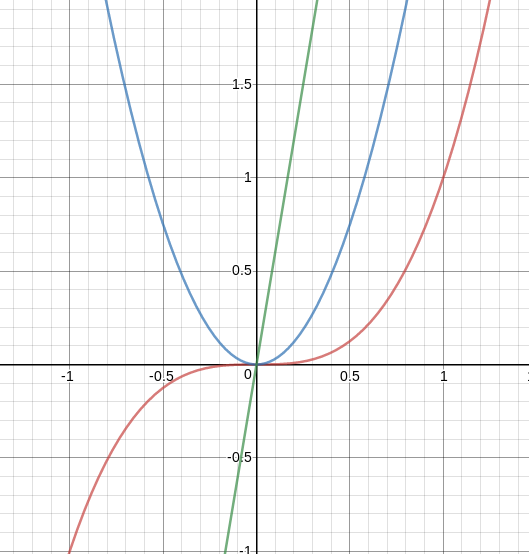
\includegraphics[width=8cm]{position_velocity_acceleration_1.png}
\end{center}
\end{figure}

\item 
\begin{figure}[h]
\begin{center}
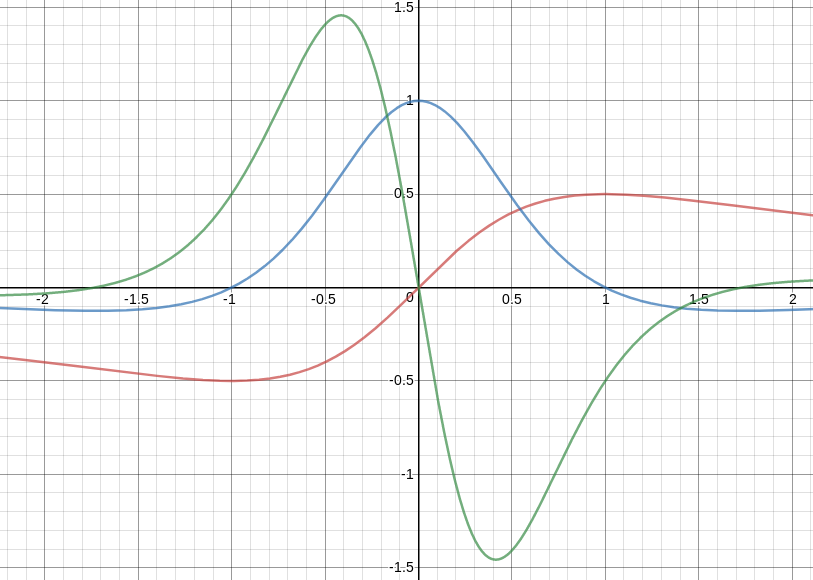
\includegraphics[width=8cm]{position_velocity_acceleration_2.png}
\end{center}
\end{figure}
\end{enumerate}


\noindent \textbf{Problem Set 2:} Find the first and second derivatives of the following functions.
\begin{enumerate}[1.]
\item $g(x)=\frac{\cos x}{\sin^2 x}$.
\item $f(x)=(\sin x + \cos x) \sec x$.
\item $r(\theta)=2\sin \theta \cos \theta$.
\item $V(r)=\frac{r^2 \cos \theta_0}{(1-r^3)^3}$.
\item $x(t)=\frac{1}{2}+\frac{\sqrt{2}}{2}\cos t + \frac{\sqrt{2}}{2} \sin t$.
\item $u(v)=\cos v \sin^2 v (v^3+v^2+v+1)$.
\end{enumerate}

\subsection{The Chain Rule}

We're onto the last of the derivative rules.  The chain rule is super important, and it also shows up more often than essentially anything else.  I'd argue that we, in some sense, already know how to do this.  Let's start with an example where we don't need it (note that in a few earlier exercises I brought this up without being too explicit about it).

\begin{example}
Imagine you have a topographical map telling you the height $y$ at a given horizontal position $x$.  This means that we can think of this map as a function $y(x)$ (fun fact, functions are often called maps).  This is nothing new!  Let's change that.

Now, imagine you also know your horizontal position $x$ as a function of time.  This gives us another function $x(t)$.  Notice that we can make a composite function $y(x(t))$ which tells us our height at a given time.  

We're now interested in finding the change in height with respect to time.  In other words, we want the derivative of $y$ with respect to $t$, but this means we must learn how to handle differentiating composite functions.
\end{example}

\begin{example}
Let's do an explicit calculation.  Let our horizontal position function $x(t)$ be given by $x(t)=2t$.  Let's let our height function $y(x)$ be given by $y(x)=x^2$.  Write down the composite function.
\vspace*{3cm}\\

Given this composite function, we can find $\frac{d}{dt} y(x(t))$ without knowing any new rules! Answer this: How does $\frac{d}{dt} y(x(t))$ relate to $y'(x)$ and $x'(t)$?
\vspace*{4cm}\\
\end{example}

\begin{remark}
Notice that $y'(x)=2x$ and that $x'(t)=2$.  Now, substitute our expression $x(t)$ in for $x$ and we find that we get $y'(x(t))=4t$.  Finally, $y'(x(t))x'(t)=\frac{d}{dt}y(x(t))$.  Maybe this seems odd, maybe it immediately makes sense.  Either way let's try to explain what's happening.
\end{remark}

\begin{remark}
Why? Why is the derivative of composite functions coming out like this:
\[
\frac{d}{dt} y(x(t)) = y'(x(t))x'(t)?
\]
Well, if we think about our specific example, $x(t)=2t$ just means we're letting our input to $y$ vary twice as fast as it regularly would.  If our input $x$ is changing twice as fast compared to normal, then our function changes in response to this, right? So it makes sense that the derivative of $x(t)$ should influence the derivative of $y(x(t))$.  Then, of course, the derivative of $y$ itself has to matter too.
\end{remark}

\begin{theorem}[(The Chain Rule)]
If $f(u)$ is differentiable at the point $u=g(x)$, and $g(x)$ is differentiable at $x$, then the composite function $(f\circ g)(x)=f(g(x))$ is differentiable at $x$ and
\[
(f\circ g)'(x)=f'(g(x))g'(x).
\]
In slightly different notation, if $y=f(u)$ and $u=g(x)$, then
\[
\frac{dy}{dx}=\frac{dy}{du}\frac{du}{dx}.
\]
\end{theorem}

\begin{remark}
You may be inclined to cancel the $du$ in the denominator with the $du$ in the numerator.  This doesn't work this way.  Why? That's a truly excellent question.  It's because the objects $du$, $dx$, and $dy$ are not numbers, or anything we're equipped to deal with.  

It's easy to make them sound scary: $du$, $dx$, and $dy$ are called \emph{one forms} and they are smooth sections of the cotangent bundle of a differentiable manifold. \emph{Note: This fact will NEVER come up in our exams or anything.  It's something you see when you go much MUCH further in math!} 
\end{remark}

\begin{remark}
Maybe it's worth reminding ourselves when we can actually compose two functions.  Remember, if we have a function $f$ and another function $g$, and we wish to make a composite of these two functions $f\circ g$, then the range of $g$ must agree with the domain of $f$. 

Letting the domain of $g$ be $D$ and the domain of $f$ be $D'$, we must have the following:
\begin{center}
\begin{tikzcd}
D \arrow[r, "g", bend left] \arrow[rr, "f\circ g"', bend right] & D' \arrow[r, "f", bend left] & R
\end{tikzcd}
\end{center}
Peeling apart this diagram, we realize that the domain of $f$ must agree with the range of $g$.  It's possible that $f$ has a domain that is strictly bigger than the range of $g$, but the domain of $f$ should not be smaller than the range of $g$! If this happens, it's possible to feed $g$ an input that will make $g$ output a value not in the domain of $f$, and poor $f$ won't know how to handle this!
\end{remark}

In the wise words of Richard Feynman, let's ``shut up and calculate!"

\begin{example}
Let $x(t)=\cos (\omega t+\delta)$.  Find $x'(t)$. 
\begin{solution}
Now note that we can write this as a composite function.  Let $u(t)=\omega t + \delta$.  Then we have 
\[
x=\cos (u).
\]
Then we find
\begin{align*}
\frac{dx}{du}&=-\sin (u)\\
\frac{du}{dt}&=\omega.
\end{align*}
This means
\begin{align*}
x'(t)=\frac{dx}{du}\frac{du}{dt}&= -\sin(\omega t + \delta)\cdot \omega. 
\end{align*}
Compare this with the notes from the previous section.
\end{solution} 
\end{example}

\begin{exercise}
Let $x(t)=\tan (t^2+t+1)$. Find $x'(t)$.
\begin{solution}~
\vspace*{6cm}
\end{solution}
\end{exercise}


\begin{exercise}
Show that the derivative of $g(t)=\tan(5-\sin 2t)$ is $g'(t)=-2(\cos 2t) \sec^2(5-\sin 2t)$. \emph{Note: this requires a ``double" chain rule!}
\begin{solution}~
\vspace*{6cm}
\end{solution}
\end{exercise}

\begin{exercise}
Let $f(u)=u^n$, where $u$ is a function of $x$.  Find $\frac{d}{dx} f(u)$.  \emph{Note: this is a nice generalization of the power rule.}
\begin{solution}~
\vspace*{6cm}
\end{solution}
\end{exercise}

\pagebreak

\noindent \textbf{\large{Worksheet: All Kinds of Derivatives, and Their Graphs}}\\


\noindent Let me introduce some important terminology when it comes to graphs of derivatives.  For all of the following we will make a necessary assumption that $f(x)$ is a function that is (at least) twice differentiable.  Meaning we have $f''(x)$ exists. Then the following apply.

\begin{definition} 
\begin{enumerate}[1.]
\item $f(x)$ is \emph{increasing on $[a,b]$} if for $c,d \in [a,b]$ and $c<d$ we have $f(c)< f(d)$.
\item $f(x)$ is \emph{decreasing on $[a,b]$} if for $c,d \in [a,b]$ and $c<d$ we have $f(c)> f(d)$.
\item If $f'(x)=0$ we say that $x$ is a \emph{critical point} of $f$.
\end{enumerate}
\end{definition}


\begin{theorem} The following are immediate results from the above definitions:
\begin{enumerate}[1.]
\item If $f'(x)>0$ then $f$ is increasing at $x$. 
\item If $f'(x)<0$ then $f$ is decreasing at $x$.
\end{enumerate}
\end{theorem}

Note that for the above, if we replace $f$ with $f'$ and $f'$ with $f''$, this is still true. 


The following are definitions that are helpful to have in the back of your mind now, but are not ones to use on Exam 2.
\begin{definition}
\begin{enumerate}[1.]
\item If $f''(x)>0$ for $x\in [a,b]$ then we say $f$ is \emph{concave up} on $[a,b]$.
\item If $f''(x)<0$ for $x\in [a,b]$ then we say $f$ is \emph{concave down} on $[a,b]$.
\item If $f''(x)=0$ we say that $x$ is an \emph{inflection point}.
\end{enumerate}
\end{definition}

If you can understand how the relations between positive/negative values, increasing/decreasing, and concave up/down for $f$ and its derivatives $f'$ and $f''$, you should be able to identify graphs much more easily.

\begin{exercise}
Is it possible for a function to be concave down and increasing? How about convave up but decreasing? Provide examples or explain why it is not possible.
\vspace*{5cm}
\end{exercise}

\begin{exercise}
Let $f(x)=x^3$. After drawing the graph of $f$, discuss everything you can about increasing/decreasing as well as concavity.  Note if there are any inflection points, and where they are.
\vspace*{7cm}
\end{exercise}

\begin{exercise}
Using this knowledge developed here, go back to the graphs from the previous day and explain which functions are $f$, which are $f'$, and which are $f''$.
\end{exercise}

\begin{exercise}
Is it possible for there to be an inflection point $x$ for $f$ where $f'(x)>0$.  How about if $f'(x)<0$.  Provide examples, or explain why it is not possible.
\vspace*{5cm}
\end{exercise}

\pagebreak

\noindent \textbf{Problem Set:} Given the functions $f$, compute their derivatives $f'$. You may want to use a separate piece of paper.
\begin{enumerate}[1.]
\item $f(x)=2x \cos (2x)$.
\item $f(x)=\cos^3(x^3)\sin x$.\\
\item $f(x)=\frac{(1+x^4)^{16}}{\sec x}$.
\item $f(x)=\frac{t^2(x+t)^2}{\cos t \sin x}$.
\item $f(x)=\left( \frac{ (x^2+x)\tan x}{x+1} \right)^2$.
\item $f(x)= \sin(\sin(\sin(x)))$.
\item $f(x)= \sin\left( \frac{\log t \frac{1}{x}}{\frac{1}{x^2}} \right)$.
\item $f(x)= \pi r^2 \cot{c}$.
\item $f(x)=\cot(\tan (x^{233}))$.
\item $f(x)= \sin \left( \frac{ \sin x}{x^3+3x^2+3x+1} \right)$.
\item $f(x)= \sin^n x$.
\end{enumerate}


\subsection{Implicit Differentiation}

Up until this point we have thought of functions as being given by an equation $y=f(x)$.  However, this isn't always possible!  Sometimes, we want to consider different equations in the plane, like $y^2=x$.  We'll make some tools to be able to do what we've been doing with functions with other equations.  

\noindent \textbf{Implicit Differentiation:}
We'll pretend that $y$ is a function of $x$.  Then we can take derivatives in the normal way.  We just have to be a bit more careful.  Let's look at some examples.

\begin{example}
How can we take the derivative of the following:
\[
x^2+y^2=1.
\]
Well, if $y$ is a function of $x$, we just apply the derivative operator $\frac{d}{dx}$ to this equation. So we have
\begin{align*}
\frac{d}{dx} (x^2+y^2)&=\frac{d}{dx} 1\\
2x+2y\frac{dy}{dx}&= 0.
\end{align*}
Believe it or not, that's it.  Just notice the use of the chain rule for $y$.
\end{example}

\begin{example}
Considering the same function, $x^2+y^2=1$. Draw the graph below:
\vspace*{5cm}\\

Now, what is the slope of the tangent line at the point $\left(\frac{\sqrt{2}}{2},\frac{\sqrt{2}}{2}\right)$? Well we can solve for $\frac{dy}{dx}$ then plug in our point.  So we get
\begin{align*}
2x+2y\frac{dy}{dx}&=0\\
\frac{dy}{dx}&=-\frac{x}{y}.
\end{align*}
Pluggin in our point tells us that $\frac{dy}{dx}=-1$, and this is the slope of the tangent line at the point of interest.  
\end{example}

\begin{question}
What happens when we consider the points $(1,0)$ and $(-1,0)$?
\vspace*{3cm}\\
\end{question}

\subsubsection{Derivatives of Higher Order}

Not too much changes if we consider derivatives of higher order. Let's just see how this works.

\begin{example}
Consider $2x^3-3y^2=8$. We wish to find $\frac{d^2 y}{dx^2}$.  So we first differentiate once,
\begin{align*}
\frac{d}{dx}(2x^3-3y^2)&=\frac{d}{dx}8\\
6x^2-6y\frac{dy}{dx}&=0\\
6x^2-6yy'&=0.
\end{align*}
Remember, $y'$ is just nice notation for $\frac{dy}{dx}$. We find that 
\begin{align*}
y'&=\frac{x^2}{y}.
\end{align*}
Now we differentiate again and find
\begin{align*}
y''&=\frac{d}{dx}\left( \frac{x^2}{y}\right) = \frac{2xy-x^2y'}{y^2}.
\end{align*}
We then substitute the known value of $y'$ to get
\begin{align*}
y''&=\frac{2xy-x^2\frac{x^2}{y}}{y^2}.
\end{align*}
Thats it!
\end{example}

\subsubsection{Tangents and Normals}

We are capable of finding tangents for graphs given by equations that aren't necessarily functions.  We're going to take this geometrical perspective a bit further.  

\begin{definition}
The \emph{normal} of a surface (curve) at a point is the line that is perpendicular (orthogonal) to the tangent line passing through that point.
\end{definition}

\begin{exercise}
Given the line $y=\frac{1}{2}x$. What is the line that is perpendicular to this?
\vspace*{3cm}\\
\end{exercise}

\begin{example}
Given the equation $x^3+y^3-9xy=0$, we want to find the tangent and normal to the curve at the point $(2,4)$.  First, we must check if $(2,4)$ is even on this curve! To see this, just plug in the $x$ and $y$ values.
\begin{align*}
x^3+y^3-9xy&=0\\
(2)^3+(4)^3-9(2)(4)&=8+64-72=0.
\end{align*}
So yes, this point is on the curve. Now, I'll let you do the work to find $\frac{dy}{dx}$. 
\vspace*{6cm}\\
You should have found that the tangent line through the point $(2,4)$ is $y=\frac{4}{5}x+\frac{12}{5}$.  What is the normal?
\vspace*{3cm}
\end{example}

\section{Applications of Derivatives}

Some of this stuff has been touched on before, but now we can treat these topics with more rigor.  We'll begin with extreme values.

\subsection{Extreme Values of Functions}

Sometimes the domain of the functions we are considering are not so important.  However, for extrema, they will be.  So please keep this in mind when you are trying to find answers.  Let's begin with the easiest type of extreme values.

\begin{definition}
Let $f$ be a function with domain $D$. Then $f$ has an \emph{absolute maximum} value on $D$ at a point $c$ if
\[
f(x)\leq f(c) ~~~~ \textrm{for all $x \in D$}.
\]
Similarly, $f$ has an \emph{absolute minimum} value on $D$ at $c$ if
\[
f(x)\geq f(c) ~~~~ \textrm{for all $x\in D$}.
\]
We then say that these absolute extrema above are \emph{global} maxima or minima. 
\end{definition}

\begin{remark}
The idea of local and global is a big one in mathematics (specifically calculus).  As we've noticed, calculus is very strong for telling us local information about functions, i.e., you can find tangent lines at single points, and tell if a function is increasing/decreasing in a small area.  

As a big side note: Topology is a field in math that is very considered with global structure whereas analysis and geometry tend to be concerned with local structure.  Fun!
\end{remark}

\begin{remark}
I invite you to go back through our notes and find where we have talked about this before.  Since we have, I will not be too concerned with overdoing examples we've already done.
\end{remark}

\begin{theorem}[(Extreme Value)]
If $f$ is continuous on a closed interval $[a,b]$, then $f$ attains both an absolute maximum value $M$ and an absolute minimum valu $m$ in $[a,b]$. That is, there are numbers $x_1$ and $x_2$ in $[a,b]$ with $f(x_1)=m$ and $f(x_2)=M$, and $m\leq f(x) \leq M$ for every $x\in [a,b]$.
\end{theorem}

\begin{remark}
This is actually a specific case of a much more general theorem, so allow me to ask a question that gets at that.
\end{remark}

\begin{question}
Let $f$ be continuous on the domain $[a,b] \cup [c,d]$.  Does $f$ attain an absolute maxima and an absolute minima?
\vspace*{2cm}\\
\end{question}

\begin{remark}
This is fact true if we take finite unions of closed intervals as well.
\end{remark}

\subsubsection{Local Extreme Values}

Since we have the wonderful tool that is the derivative, we have the ability to look at local extrema.  This is what we'll do now.

\begin{definition}
A function $f$ has a \emph{local maximum} value at a point $c$ within its domain $D$ if $f(x)\leq f(c)$ for all $x\in D$ lying in some open interval containing $c$.  This is to say that there exists a $\delta>0$ so that for $x\in (c-\delta, c+\delta)$ we have $f(x)\leq f(c)$.

A function $f$ has a \emph{local minimum} value at a point $c$ within its domain $D$ if $f(x)\geq f(c)$ for all $x\in D$ lying in some open interval containing $c$. This is to say that there exists a $\delta>0$ so that for $x\in (c-\delta, c+\delta)$ we have $f(x)\geq f(c)$.
\end{definition}

It's worth noting that local extrema are sometimes referred to as \emph{relative extrema}. I will likely not use that terminology, but you should be aware of this.

\begin{example}
Let's take a look at the following graph and discuss the extrema we see.  We will also take note of what's going on at these points as far as the derivative.
\vspace*{6cm}\\
\end{example}

\subsubsection{Finding Extrema}

\begin{theorem}[(The First Derivative Theorem for Local Extreme Values)]
If $f$ has a local maximum or minimuim value at an interior point $c$ of its domain, and if $f'$ is defined at $c$, then
\[
f'(c)=0.
\]
\end{theorem}

\begin{question}
As with any logical statement, we should consider the opposite direction.  So, if $f'(c)=0$, is $f(c)$ a local max or min for $f$? If yes, why? If not, can you give a good counter example?
\vspace*{3cm}\\
\end{question}

\begin{definition}
A point $x$ of the domain $D$ of a function $f$ where $f'(x)=0$ or where $f'(x)$ is undefined or where $x$ is at the endpoint of an interval in the domain is called a \emph{critical point}. 
\end{definition}

\begin{example}
Let's see what these look like.  Consider the following graph:
\vspace*{6cm}\\
\end{example}

\noindent \textbf{How to find absolute extrema of a continuous function $f$ on a finite closed interval:} 
\begin{enumerate}[1.]
\item Evaluate $f$ at all the critical points.
\item Take the largest and smallest of these values.
\end{enumerate}

\begin{exercise}
Find the absolute maximum and minimum values of $g(t)=8t-t^4$ on $[-2,2]$. First, try to graph the function, then use the tools we just developed.
\vspace*{6cm}\\
\end{exercise}

\subsection{The Mean Value Theorem}

The mean value theorem (which we're about to cover) is a very important result in calculus.  It may seem a bit surprising at first, but the more you look at it, the more natural it gets. It should feel very similar to the intermediate value theorem!

\begin{theorem}[(Rolle's Theorem)] 
Suppose that $y=f(x)$ is continuous over the closed interval $[a,b]$ and differentiable at every point of its interior $(a,b)$. If $f(a)=f(b)$, then there is at least one number $c\in (a,b)$ such that $f'(c)=0$.
\end{theorem}

\begin{example}
We'll look at proving this in a ``morally" correct way.  That is, by drawing a function satisfying the criteria, and seeing that this definitely holds true. You're invited to come up with a case where it isn't!
\vspace*{6cm}\\
\end{example}

\begin{example}
Here is a useful application of Rolle's theorem with the intermediate value theorem. First, recall what the intermediate value theorem is, and write it below:
\vspace*{3cm}\\
Now, we want to show that the equation $f(x)=x^3+3x+1$ has one real root (i.e., $f(x)=0$ for one real $x$). 
\begin{solution}
Note that $f(-1)=-3$ and that $f(0)=1$. The continuity of $f$ implies that there is some value $c\in (-1,0)$ so that $f(c)=0$.  This gives us that there exists one real solution.  Now, we didn't use Rolle's theorem yet, but that will tell us that there is in fact just this single real solution. Let's see how:

Suppose there were at least two solutions, one being $c$ that we just found and another being $d$. That would mean that there is some point $x$ between $c$ and $d$ such that $f'(x)=0$.  But $f'(x)=3x^2+3$ is never zero! Hence, the only possible real solution is $c$.
\end{solution}
\end{example}


\begin{remark}
Sometimes when we're learning new mathematics, we must learn a few lies at first.  This is why we are saying things like one \emph{real} solution. If we work over the complex number system $\mathbb{C}$, then there will always be $n$ roots to an $n$th degree polynomial.  This is \emph{fundamental theorem of algebra}.
\end{remark}

As it turns out, Rolle's theorem is a special case of a more general theorem.  This more general theorem is what we'll do right now!

\begin{theorem}[(The Mean Value Theorem)]
Suppose $y=f(x)$ is continuous over a closed interval $[a,b]$ and differentiable on $(a,b)$. Then there is at least one point $c\in (a,b)$ such that
\[
\frac{f(b)-f(a)}{b-a}=f'(c).
\]
\end{theorem}

\begin{example}
We'll again prove this by picture.  Let's take a look:
\vspace*{6cm}\\
\end{example}

\begin{question}
What is a good physical interpretation of this problem?\\

\noindent \emph{Answer:} Think about driving a car.  If your average speed over some time was 50$[mph]$, then you certainly had to have been going 50$[mph]$ at some moment in time! This is the premise of the average speed traps used in some places.
\end{question}

\begin{remark}
The mean value theorem can be even further generalized in other ways.  It's pretty fascinating really. For example, similar results hold true in higher dimensions. 
\end{remark}

\subsubsection{Consequences of MVT}

\begin{corollary}
If $f'(x)=0$ at each point $x$ in an open interval $(a,b)$, then $f(x)=C$ for all $x\in (a,b)$, where $C$ is a constant.
\end{corollary}

\begin{remark}
What this is saying is going to become more clear with the next corollary.
\end{remark}

\begin{corollary}
If $f'(x)=g'(x)$ at each point $x$ in an open interval $(a,b)$, then there exists a constant $C$ such that $f(x)=g(x)+C$ for all $x\in (a,b)$. That is $f-g$ is a constant function on $(a,b)$.  
\end{corollary}

\begin{example}
Let's see this with a picture as well. 
\vspace*{6cm}\\
\end{example}

\begin{remark}
To me, this $+C$ result is fairly important.  In the realm of field theory, when this type of thing shows up, it's telling of more underlying structure occuring.  Of course, this shows up in ways that are a bit more complicated, but the idea is extremely analogous. The idea I'm talking about here is called \emph{gauge theory}.  All of the important physical theories in physics (to me) are gauge theories.  

In MATH 261, you will be talking about electric fields (though you may not mention them), and you'll find these fields are what we see as ``real." However, there is an underlying potential that you can find the electric field from and this is called the \emph{voltage}. This voltage is defined up to an additive constant called a gauge.  It's similar with the magnetic field, except this additive constant (gauge) is written a bit differently. Also the magnetic potential is a bit more complicated than the voltage. However, the electric and magnetic fields are all actually part of the same field, and are just the same via another gauge (Lorentz gauge) thanks to special relativity.  If you read all of this, I'm proud! Enough digression on things I like, let's get back to math.
\end{remark}

\begin{example}
Let's use what we just learned to solve a problem from real life.  Let's assume an object is falling freely from rest with the usual gravitational acceleration of $9.8[ms^{-2}]$. We'll assume the position $x(t)$ is measured from the starting position and pointing down (i.e, falling 5$[m]$ will mean $x=5$). 

We know that $v(t)=9.8t+C$ based on our previous examples.  Now, this $C$ can be determined since we said that we started at time $t=0$ from rest. This means $v(0)=0=9.8(0)+C$.  Thus, $C=0$. 

Then $x(t)=4.9t^2+C$ as well. But we started at $t=0$ and said our starting point was where we measure from, meaning that $x(0)=4.9(0)^2+C=0$ meaning that $C=0$ again.
\end{example}

\subsection{Monotonic Functions and the First Derivative Test}

We'll spend a bit more time talking about increasing and decreasing functions.  There's a few more things that should be said.

\begin{definition}
A function that is increasing or decreasing on an interval is said to be \emph{monotonic} on the interval.
\end{definition}

\begin{corollary}
Suppose that $f$ is continuous on $[a,b]$ and differentiable on $(a,b)$. Then if $f'(x)>0$ at each point $x\in (a,b)$, then $f$ is increasing on $[a,b]$.  Similarly, if $f'(x)<0$ at each point $x\in (a,b)$, then $f$ is decreasing on $[a,b]$.
\end{corollary}

\begin{remark}
It's worth noting that the reverse of the above statements is not necessarily true.  For example, $f(x)=x^3$ is always increasing yet $f'(0)=0$.
\end{remark}

\begin{question}
Why do we require continuity on $[a,b]$ and differentiability on $(a,b)$?
\vspace*{2cm}\\
\end{question}

\begin{example}
Let's find which intervals in which $f(x)=x^3-12x-5$ is increasing and decreasing. We first find
\begin{align*}
f'(x)=3x^2-12=3(x+2)(x-2).
\end{align*}
Notice $f'$ is zero when $x=\pm 2$.  We need just check the sign of $f'$ in the intervals $(-\infty,-2)$, $(-2,2)$, and $(2,\infty)$. We find that $f'$ is positive in $(-\infty, -2)$ (meaning $f$ is increasing), $f'$ is negative in $(-2,2)$ (meaning $f$ is decreasing) and $f'$ is positive in $(2,\infty)$ (meaning that $f$ is increasing). A drawing and a chart like below may be helpful!
\vspace*{7cm}\\ 
\end{example}

\begin{question}
How can we know when a function is still increasing or decreasing when the derivative is zero?
\vspace*{2cm}\\
\end{question}

\noindent\textbf{First Derivative Test for Local Extrema:} Suppose that $c$ is a critical point of a continuous function $f$, and that $f$ is differentiable at every point in some interval containing $c$ except possibly at $c$ itself. Moving across this interval from left to right,
\begin{enumerate}[1.]
\item if $f'$ changes from negative to positive at $c$, then $f$ has a local minimum at $c$;
\item if $f'$ changes from positive to negative at $c$, then $f$ has a local maximum at $c$;
\item if $f'$ does not change sign at $c$ (that is, $f'$ is positive on both sides of $c$ or negative on both sides), then $f$ has no local extremum at $c$.
\end{enumerate}

\begin{example}
Let's look at a graph displaying all these options.
\vspace*{7cm}\\
\end{example}

\begin{exercise}
Within the interval $0\leq x \leq 2\pi$, find the critical points of 
\[
f(x)=\sin^2 x - \sin x -1.
\]
Identify the open intervals on which $f$ is increasing and decreasing. Find the function's local and absolute extreme values.
\vspace*{7cm}\\
\end{exercise}

\subsection{Concavity and Curve Sketching}

Luckily we already talked a small bit about concavity, so this won't be totally new to us! Our goal is to be able to understand as much as we can about the shape of a function based off of information given to us by first and second derivatives.  Last time we concentrated on first derivatives and now we'll get to the second derivatives.

Let's start with some basic definitions.

\begin{definition}
The graph of a differentiable function $y=f(x)$ is
\begin{enumerate}[(a)]
\item \emph{concave up} on an open interval $I$ if $f'$ is increasing on $I$. 
\item \emph{concave down} on an open interval $I$ if $f'$ is decreasing on $I$.
\end{enumerate}
\end{definition}

We need a picture to really see what is going on here.  I'll leave some room for this.
\vspace*{5cm}\\

It's likely helpful to think of parabolas as being the generic idea of concave up and concave down.  What I mean is that if something is concave up, locally it looks somewhat like an upward opening parabola and it is a similar story for concave down.

\begin{remark}
Keep in mind we are \underline{not} talking about the sign of $f'$ in this case.  Rather, we are concerned with the monotone nature of $f'$.  This should make you think of taking another derivative and checking that sign!
\end{remark}

\noindent \textbf{The Second Derivative Test for Concavity:} Let $y=f(x)$ be twice-differentiable on an open interval $I$.
\begin{enumerate}[1.]
\item If $f''>0$ on $I$, the graph of $f$ over $I$ is concave up.
\item If $f''<0$ on $I$, the graph of $f$ over $I$ is concanve down.
\end{enumerate}

\begin{definition}
A point $(c,f(c))$ where the graph of a function has a tangent line and where the concavity changes is an \emph{inflection point}.
\end{definition}

\begin{proposition}
An inflection point occurs at $(c,f(c))$ if $f''(c)=0$ or $f''(c)$ fails to exist.
\end{proposition}

It's worthwhile to do a few examples now.  

\begin{example}
Consider $f(x)=x^{5/3}$. It looks like:
\vspace*{4cm}\\
Note that $f'(0)=0$ but $f''(0)$ is not defined.  Yet for $x<0$ we have $f''(x)<0$ and for $x>0$ we have $f''(x)>0$.  So $x=0$ is an inflection point for this function.
\end{example}

\begin{example}
Consider $f(x)=x^4$.  It looks like:
\vspace*{4cm}\\
Note that $f''(0)=0$ yet this function is always concave up.  Remember, it looks essentially like an upward opening parabola.
\end{example}

\begin{example}
Consider $f(x)=x^{1/3}$. It looks like:
\vspace*{4cm}\\
Note that at $x=0$, $f'(x)$ and $f''(x)$ both fail to exist.  Yet, you can check that $x=0$ is an inflection point.
\end{example}

\noindent \textbf{Second Derivative Test for Local Extrema:} Suppose $f''$ is continuous on an open interval that contains $x=c$. 
\begin{enumerate}[1.]
\item If $f'(c)=0$ and $f''(c)<0$, then $f$ has a local maximum at $x=c$.
\item If $f'(c)=0$ and $f''(c)>0$, then $f$ has a local minimum at $x=c$.
\item If $f'(c)=0$ and $f''(c)=0$, then the test fails. The function $f$ may have a local maximum, a local minimum, or neither.
\end{enumerate}

\begin{exercise}
Consider $f(x)=x^4-4x^3+10$.  Find the critical points, inflection points and the local and absolute extreme values.
\vspace*{10cm}\\
\end{exercise}

\begin{remark}
You should try to reconcile this second derivative test for local extrema to what we mentioned previously with the first derivative test! Go back and check the examples and exercises with these new rules.
\end{remark}

We will move on to doing many examples with this and doing some curve sketching as well.\\

\noindent \textbf{Procedure for Graphing $y=f(x)$}
\begin{enumerate}[1.]
\item Identify the domain of $f$ and any symmetries the curve may have.
\item Find the derivatives $y'$ and $y''$.
\item Find the critical points of $f$, if any, and identify the function's behavior at each one.
\item Find where the curve is increasing and where it is decreasing.
\item Find the points of inflection, if any occur, and determine the concavity of the curve.
\item Identify any asymptotes that may exist.
\item Plot key points, such as the intercepts and the points found in Steps 3-5, and sketch the curve together with any asymptotes that exist.
\end{enumerate}

\begin{example}
Sketch the grpah of $f(x)=\frac{(x+1)^2}{1+x^2}$.\\
\noindent \emph{Solution:}~
\begin{enumerate}[1.]
\item The domain of $f$ is $(-\infty, \infty)$ and there are no symmetries no use.
\item First we find $f'$.
\begin{align*}
f'(x)&=\frac{(1+x^2)\cdot 2(x+1)-(x+1)^2\cdot 2x}{(1+x^2)^2}\\
&=\frac{2(1-x^2)}{(1+x^2)^2}.
\end{align*}
Then we find $f''$.
\begin{align*}
f''(x)&=\frac{(1+x^2)^2\cdot 2(-2x)-2(1-x^2)[2(1+x^2)\cdot 2x]}{(1+x^2)^4}\\
&= \frac{4x(x^2-3)}{(1+x^2)^3}.
\end{align*}
\item The critical points are $x=\pm 1$ where $f'(x)=0$ since $f'$ exists everywhere in the domain. At $x=-1$ we have that $f''(-1)=1>0$, which means that this is a local minimum by the Second Derivative Test. At $x=1$, $f''(1)=-1<0$ which means that this is a local maximum by the Second Derivative Test.
\item We check each interval beginning with $(-\infty,-1)$. Note that $f'(x)<0$ on this interval so the curve is decreasing. On $(-1,1)$ we have $f'(x)>0$ and so the curve is increasing. Lastly, on $(1,\infty)$ we have $f'(x)<0$ so the curve is decreasing.
\item We have that the denominator of $f''$ is always positive so we look for when the numerator will be zero.  This happens at $x=-\sqrt{3},0$ and $\sqrt{3}$. 

Checking the intervals $(-infty, -\sqrt{3})$ we see that $f''(x)<0$ here. On $(-\sqrt{3},0)$ we have that $f''(x)>0$. On $(0,\sqrt{3})$ we have that $f''(x)<0$. Lastly, on $(\sqrt{3},\infty)$ we note that $f''(x)>0$. So each one of these points is an inflection point. These signs of $f''$ also tell us the concavity in those regions.
\item To view asymptotes, note that there are no vertical asymptotes since there is no point where $f(x)$ approaches $\pm \infty$. So we just want to check the behavior as $x\to \pm \infty$ to see if there are horizontal aysmptotes. We have
\begin{align*}
f(x)&=\frac{(x+1)^2}{1+x^2}=\frac{x^2+2x+1}{1+x^2}\\
&=\frac{1+(2/x)+(1/x^2)}{(1/x^2)+1}.
\end{align*}
Then as $x\to \infty$ we see that $f(x)\to 1^+$. As $x\to -\infty$ we find that $f(x)\to 1^-$.
\item We draw the graph taking note of all the information we just found.
\vspace*{5cm}\\
\end{enumerate}
\end{example}

\begin{exercise}
Sketch the graph of $f(x)=\frac{x^2+4}{2x}$.  
\vspace*{10cm}\\
\end{exercise}

\begin{exercise}
Draw a function $f$ satisfying the following criteria:
\begin{enumerate}[(i)]
\item $\lim_{x\to -\infty} f(x)=-\infty$.
\item $f$ is concave down on $(-\infty, -3)$.
\item $f''(-2)<0$ and $f'(-2)=0$.
\item $f$ has an inflection point at $x=-2$.
\item On $(-2,1)$, $f$ is concave up.
\item $f$ has a local minima at $x=-1$.
\item $f''(1)=0$.
\item On $(1,2)$, $f''<0$.
\item $f'(2)=0$.
\item On $(2,3)$, $f$ is concave down.
\item $f$ has an inflection point at $x=3$.
\item $f$ retains the same concavity from $(3,\infty)$ and $\lim_{x\to \infty} f(x)=1^+$.
\end{enumerate}
\vspace*{6cm}
\end{exercise}

\subsection{Applied Optimization}

We've reached a big milestone here.  At this point, we'll start to see some of the real usefulness of calculus.  We'll work through a lot of real life examples and I'll try to motivate important problems that are a bit more general than what we do here.

Where is optimization used?  Simply put: everywhere.  Any time you're doing anything, you're usually trying to do it in the fastest, easiest, or least painful way.  That's the goal here.  Out in industry? Well, profit maximization and machine learning are two HUGE examples.  Optimization is useful in pure mathematics, physics, economics, and business.

Here are a few canonical examples:

\begin{enumerate}[1.]
\item Given so many feet of fencing material, what is the largest yard you can fence in?
\item What is the shortest distance between two points?
\item What is the best price to sell this item for in order to make the most profit?
\item What is the best way to maximize strength and minimize weight given some constraints?
\end{enumerate}

Our book gives us this outline of steps for solving optimization problems.  They are as follows:

\noindent \textbf{Solving Applied Optimization Problems:}
\begin{enumerate}[1.]
\item Read and understand the problem. Know what quantity needs to be optimized and what your constraints are.
\item Draw pictures!
\item Create variables for each quantity that is not yet determined.  
\item See how these variables relate to each other and create an equation.
\item Test for critical points in order to find the extreme values for this function.
\end{enumerate}

\begin{example}
An open-top box is to be made by cutting small congruent squares from the corners of a 1$[ft.]$ by $1[ft.]$ square shit of tin and bending up the sides. How large should the squares cut from the corners be to make the box hold as much as possible?

\noindent \emph{Solution:} Draw this as follows:
\vspace*{5cm}\\
Now, the volume of this box will follow the equation
\[
V(x)=x(12-2x)^2=144x-48x^2+4x^3.
\]
The amount we can cut is $0[in.]\leq x\leq 6[in.]$ due to the side lengths of the tin. On this interval, the graph looks like
\vspace*{5cm}\\
Now, we have a rough idea of where the extreme values are. So we take the derivative
\begin{align*}
\frac{dV}{dx}=144-96x+12x^2=12(12-8x+x^2)=12(2-x)(6-x).
\end{align*}
We then get that the zeros are $x=2$ and $x=6$.  This makes the list of critical points $x=0$, $x=2$, and $x=6$. We plug these into the original function.
\begin{align*}
V(0)&=0\\
V(2)&=128\\
V(6)&=0.
\end{align*}
Hence, the maximum volume $128[in.^3]$. Thus we should cut out $2[in.]$ on each side.
\end{example}

\begin{exercise}
You have been asked to design a one-liter can shaped like a right circular cylinder. What dimensions will use the least material?
\vspace*{10cm}
\end{exercise}

\begin{example}[(Snell's Law of Refraction)]
Given two different media, each with a different density, we want to find the path will travel when passing between the interface of these substances. Let's first draw a picture:
\vspace*{5cm}\\

Light will choose the path between $A$ and $B$ that takes the shortest amount of time.  This optimization problem then comes down to minimizing time (or, in other words, action). We can write
\begin{align*}
\textrm{time}=\frac{\textrm{distance}}{\textrm{velocity}}.
\end{align*}  
We then have
\[
t_1 = \frac{\sqrt{a^2+x^2}}{c_1}
\]
and
\[
t_2 = \frac{\sqrt{b^2+(d-x)^2}}{c_2}.
\]
Then of course the total time is
\[
t=t_1+t_\frac{\sqrt{a^2+x^2}}{c_1}+\frac{\sqrt{b^2+(d-x)^2}}{c_2}.
\]
We then differentiate to see that
\[
\frac{dt}{dx}=\frac{x}{c_1 \sqrt{a^2+x^2}}=\frac{d-x}{c_2\sqrt{b^2+(d-x)^2}}
\]
and note that this can be written as
\[
\frac{dt}{dx}=\frac{\sin \theta_1}{c_1}-\frac{\sin \theta_2}{c_2}.
\]
At $x=0$, $\frac{dt}{dx}<0$ and for $x=d$, $\frac{dt}{dx}>0$ and so by the Intermediate Value Theorem we know there is some $x_0\in [0,d]$ such that $\frac{dt}{dx}=0$.  Then at this point we have
\begin{align*}
\frac{\sin \theta_1}{c_1}=\frac{\sin \theta_2}{c_2}.
\end{align*}
\end{example}

\section{Integrals}

Here's the idea of what is to come:

Say there is a quantity that we wish to keep track of over time.  We might ask how the quantity has accumulated over an interval of time.  This idea is captured in what is called an (definite) integral.  

Mathematically, what is an integral?  An integral is another example of an operator that eats functions and spits out a number.  Think back to when we first defined derivatives.  These were operators that took in functions and spit out a number as well.  However, we also found that we can use derivative operators to take in functions and spit out a new function called the derivative.  We will also find that the integral mimics this in that we can tweak it slightly to give us new functions instead of just numbers.

I wish to motivate the idea of integrals from their origins in physics.  Newton was asking a few questions, and it turns out these questions are solved by integration.

\subsection{Area and Estimating with Finite Sums}

\subsubsection{Area}

Often times integrals are introduced as finding the ``area under a curve." While this isn't wrong, it fails in one respect. Namely, the idea of area does not allow for both positive and negative. When we think of area, we think of a positive number.  This is why I prefer the idea of thinking about keeping track of traveled distance.  We'll work to that.

Let's say that we want to find the area under the curve $f(x)=1-x^2$ from $x=0$ to $x=1$.  Let's take a look at this
\vspace*{5cm}\\

Just like we did for derivatives, we first want to make an approximation of this area.  The easiest possible way is to divide the domain $[0,1]$ into smaller chunks and approximate the function on these chunks to be something with an easy area to compute. The easiest area to find is that of a rectangle since the area is merely the base times the height.  Now let's draw an approximation of our function when we split the interval into two equal sized chunks $[0,1/2]$ and $[1/2,1]$. There are choices to make here. We can take an approximate the function on each interval in a few ways.  Let's concentrate on two of them for now.  We'll consider the \emph{left endpoint} and \emph{right endpoint} approximations. So here we draw this
\vspace*{5cm}\\

The area for the left endpoint approximation is
\[
A_L\approx 1\cdot \frac{1}{2} + \frac{3}{4}\cdot \frac{1}{2}=0.875
\]
and for the right endpoint approximation
\[
A_R \approx \frac{3}{4} \cdot \frac{1}{2} + 0 \cdot \frac{1}{2}=0.375.
\]
Note that the base is the same for each interval and we will often call this $\Delta x$.  Then this is multiplied by the function value at the left or right endpoint respectively.

What we now notice, is that this area under the curve $f(x)$ must be between these two estimations. The other thing to notice is that we can keep subdividing the interval $[0,1]$ and use both of these approximations to find better and better guesses at the area. If we repeated this process infinitely, we would converge to the area. This will be how we define the integral. The idea can bee seen in the following picture:
\vspace*{5cm}\\



\subsubsection{Distance Travelled}

If we want to think of the total distance travelled by a particle, then we will have to keep track of the speed of the particle at all times and try to add up distance travelled on subintervals. Let's do this with an example.

\begin{example}
Let the velocity function for a particle be $160-9.8t [ms^{-1}]$. We want to see how much the particle travels in $3$ seconds. The true answer is $435.9[m]$, and we wish to see how close we can get.\\
\noindent \emph{Solution:} First, notice that this is a decreasing function, so left endpoint approximation will give us an upper bound and the right endpoint approximation will give a lower bound. 

First we divide the interval $[0,3]$ into $[0,1]$, $[1,2]$, and $[2,3]$.  Then with the left endpoint approximation we have
\begin{align*}
D&\approx f(t_1) \Delta t + f(t_2)\Delta t + f(t_3) \Delta t\\
&= [160-9.8(0)](1)+[160-9.8(1)](1)+[160-9.8(2)](1)\\
=450.6.
\end{align*}
and for the right endpoints,
\begin{align*}
D &\approx f(t_1)\Delta t + f(t_2) \Delta t + f(t_3) \Delta t\\
&= [160-9.8(1)](1)+[160-9.8(2)](1)+[160-9.8(3)](1)\\
&= 421.2.
\end{align*}
and so the true distance satisfies
\[
421.6\leq D \leq 450.6.
\]
If we do this with 6 intervals, we find the true distance is 
\[
428.55 \leq D \leq 443.25.
\]
Doing this with 192 intervals, we find
\[
435.67\leq D \leq 436.13.
\]
As we can see, these are narrowing in on the true value of $435.9$.
\end{example}

\begin{remark}
There's something important to note here and that is that $f(t)\geq 0$ on this interval we chose.  Had it not been, we would instead need to consider $|f(t)|$ where we used it above.
\end{remark}

It is with this that we say the following:\\
\noindent The \emph{total distance travelled} is approximately
\begin{align*}
|v(t_1)|\Delta t + |v(t_2)|\Delta t + \cdots + |v(t_n)|\Delta t
\end{align*}
where $t_1$ is the initial starting point in time and $t_n$ is the ending point in time.

\subsubsection{Average Value of a Nonnegative Continuous Function}

\begin{question}
How do you compute the average value of $n$ different quantities $x_1,\dots,x_n$?
\vspace*{2cm}\\
\end{question}

The idea is that, just as we did before, we can use this to find the average value of a function.  We'll take more and more intervals, and ultimately converge to this value. 

\begin{example}
Let's estimate the average value of $\sin x$ on the interval $[0,\pi]$.  First, we draw this:
\vspace*{4cm}\\
Note that the length of the interval $[0,\pi]$ is $\pi-0=\pi$.  If we break this interval up into, say, eight peices each with length $\pi/8$, then we find that using the left endpoint approximation we have
\begin{align*}
A& \approx \left( \sin \frac{\pi}{8} + \sin \frac{\pi}{4} + \sin \frac{3\pi}{8} + \sin \frac{\pi}{2} + \sin \frac{5\pi}{8} + \sin \frac{3\pi}{4} + \sin \frac{7\pi}{8} \right) \cdot \frac{\pi}{8}\\
&\approx (0.38+0.71+0.92+1+1+0.92+0.71+0.38)\cdot \frac{\pi}{8} = (6.02)\cdot \frac{\pi}{8} \approx 2.364.
\end{align*}
Of course, we need to divide by the length of the interval in order to find the average height of the function, and so we see that
\begin{align*}
2.365/\pi \approx 0.753.
\end{align*}
The actual value is $\frac{2}{\pi}\approx 0.63662.$
\end{example}

\subsubsection{The Definite Integral}

We wish to define the following: Given a function defined on $[a,b]$, we want the net area under the curve.  We write this as
\[
\int_a^b f(x)dx.
\]
We call this the \emph{definite integral} from $a$ to $b$ of $f$ $dx$.  Here, $dx$ is just saying, ``with respect to the variable $x$." Sometimes you may see this written as
\[
\int_a^b dx f(x)
\]
or
\[
\int_a^b dx (f(x)).
\]
In this last notation, the fact that the definite integral is operating on a function is a bit more apparent.

\subsubsection{Riemann Sums}

Take an arbitrary bounded function $f$ defined on $[a,b]$. We wish to divide the interval $[a,b]$ into smaller sections so that we can approximate the net area under the curve $f$.  How do we do this? Well, we pick $n-1$ points in $(a,b)$ so that
\[
a<x_1<x_2<\cdots < x_{n-1} < b.
\]
and actually choose $x_0=a$ and $x_n=b$ so that
\[
a=x_0<x_1<x_2\cdots<x_{n-1}<x_n=b.
\]
We call the set $P=\{x_0,x_1,\dots,x_n\}$ a \emph{partition} of $[a,b]$.  Notice that this partition divides $[a,b]$ into the sub intervals
\[
[x_0,x_1],[x_1,x_2],\dots,[x_{n-1},x_n].
\]
We then define $\Delta x_k = x_k-x_{k-1}$ and define the \emph{norm} of the partition $\|P\|$ to be the largest $\Delta x_k$. 

Great, now we say that the \emph{Riemann sum for $f$ on the interval $[a,b]$} is
\[
S_p \sum_{k=1}^n f(c_k)\Delta x_k.
\]
Here, $c_k$ is just a point in the interval $[x_{k-1},x_k]$. We could pick $c_k$ to be the left or right endpoint as we've seen.


\subsubsection{Definite Integrals}

\begin{definition}
Let $f(x)$ be a function defined on $[a,b]$. We say that a number $J$ is the \emph{definite integral of $f$ over $[a,b]$} and that $J$ is the limit of the Riemann sums $\sum_{k=1}^n f(c_k)\Delta x_k$ if the following condition is satisfied:

Given any number $\epsilon>0$ there is a corresponding number $\delta>0$ such that for every partition $P=\{x_0,x_1,\dots,x_n\}$ of $[a,b]$ with $\|P\|<\delta$ and any choice of $c_k$ in $[x_{k-1},x_k]$, we have
\[
\left| \sum_{k=1}^n f(c_k)\Delta x_k - J \right| < \epsilon.
\]
\end{definition}

Well, what is this $J$? It is
\begin{align*}
J= \lim_{\|P\|\to 0} \sum_{k=1}^n f(c_k)\Delta x_k,
\end{align*}
and in fact, it is also
\begin{align*}
J=\int_a^b f(x) dx.
\end{align*}

Let us break this symbol apart a little bit before going into it some more
\vspace*{4cm}\\

Given this, we have the following definitions.
\begin{definition}~
\begin{enumerate}[1.)]
\item We say that the Riemann sums of $f$ on $[a,b]$ \emph{converge} to the definite integral $J=\int_a^b f(x) dx$.
\item We say that $f$ is \emph{integrable} over $[a,b]$.
\end{enumerate}
\end{definition}

Usually it is easiest to pick subintervals of constant width, i.e., $\Delta x = (b-a)/n$, then the Riemann sums become
\begin{align*}
S_n = \sum_{k=1}^n f(c_k)\Delta x_k = \sum_{k=1}^n f(c_k) \left( \frac{b-a}{n}\right),
\end{align*}
where $c_k$ is chosen in the $k$th interval.  It in fact, does not matter which point you choose in each interval if $f$ is integrable. When the limit as $n\to \infty$ exists, we have
\begin{align*}
J=\int_a^b f(x)dx = \lim_{n\to \infty}\sum_{k=1}^n f(c_k) \left( \frac{b-a}{n} \right).
\end{align*}
Note that $\|P\|\to 0$ is the same as $n\to \infty$ in the case where we are choosing equal length intervals.

Now, we can pick the left or right endpoint of each interval to simplify things, in which case we have the following:

\begin{align*}
\int_a^b f(x)dx = \lim_{n\to \infty} \sum_{k=1}^n f\left( a + k\frac{(b-a)}{n}\right) \left( \frac{b-a}{n}\right)
\end{align*}
for right endpoints. 

\begin{question}
What is the formula for left endpoints?
\end{question}

\begin{question}
How strong of a requirement is it of a function to be integrable? Is continuity stronger? Weaker? What about differentiability?
\end{question}

\begin{definition}
If $y=f(x)$ is nonnegative and integrable over a closed interval $[a,b]$, then the \emph{area under the curve $y=f(x)$ over $[a,b]$} is the integral of $f$ from $a$ to $b$,
\[
A=\int_a^b f(x) dx.
\]
\end{definition}

But what about for a function that has some negative values? Then we'll say the following two things.

\begin{definition}
If $y=f(x)$ is integrable over $[a,b]$, then the \emph{net area under the curve $f(x)$ over $[a,b]$} is
\[
A_{net} = \int_a^b f(x)dx.
\]
\end{definition}
You should be able to draw an example of this:
\vspace*{4cm}\\

\begin{definition}
If $y=f(x)$ is integbrable over $[a,b]$, then the \emph{total area under the curve $f(x)$ over $[a,b]$} is
\[
A_{tot} = \int_a^b |f(x)|dx.
\]
\end{definition}

The way I like to think about this is with \emph{displacement} and \emph{distance travelled}.

\begin{example}
If I run around a 400$[m]$ track starting from the start line and ending there as well, then I've had $0 [m]$ of displacement but $400[m]$ of distance travelled. Let's look at this as a graph:
\vspace*{4cm}\\
\end{example}

\subsubsection{Average Value of A Function Revisited}

Often times when computing statistics we will want to find the average value for some observable event. Performing statistical studies or measurements is certainly common, and you may be surprised how often the idea of averaging a function using an integral will come up.  Let's see how to do it.

\begin{definition}
If $f(x)$ is integrable over $[a,b]$, then the \emph{average value of $f$ on $[a,b]$} is given by
\begin{align*}
Average=\mu=\frac{1}{b-a} \int_a^b f(x)dx.
\end{align*}
Note that the average value is sometimes referred to as the \emph{mean} or even \emph{expected value}.
\end{definition}

\subsubsection{Some Common Integrals}

Eventually we will learn how to evaluate integrals in a stronger way, but for now we will stick with Riemann sums. But let's take a look at a few examples:

\begin{exercise}
Let $f(x)=c$ on the domain $[a,b]$.  What is the value of
\[
I=\int_a^b f(x)dx?
\]
\vspace*{5cm}\\
\end{exercise}

\begin{example}
Consider the function $f(x)=x$ on the domain $[-3,5]$. What is the value of
\[
I=\int_{-3}^5 f(x)dx?
\]
\noindent\emph{Solution:} First, we need to know something about integrals.  We in fact already do know this, but haven't written it down.  Namely we have the following:
\begin{align*}
I=\int_{-3}^5 f(x) dx = \int_{-3}^0 f(x) dx + \int_0^5 f(x)dx.
\end{align*}
Now, we also have this property as well:
\begin{align*}
\int_{-3}^0 f(x)dx = -\int_0^{-3} f(x)dx.
\end{align*}
So let us figure out how to integrate 
\[
\int_0^b x dx.
\]
Writing out the Riemann sums, we find the right endpoint approximation is
\begin{align*}
\int_0^b x dx &\approx \sum_{k=1}^n f(c_k)\Delta x = \sum_{k=1}^n \frac{kb}{n}\cdot \frac{b}{n}\\
&= \frac{b^2}{n^2} \sum_{k=1}^n k\\
&= \frac{b^2}{n^2} \cdot \frac{n(n+1)}{2}\\
&= \frac{b^2}{2}\left( 1+ \frac{1}{n}\right).
\end{align*}
Now notice, if we take $n\to \infty$, this is not an approximation and we have
\begin{align*}
\int_0^b x dx &= \lim_{n\to \infty} \frac{b^2}{2}\left(1+\frac{1}{n}\right)\\
&= \frac{b^2}{2}.
\end{align*}
If we use this in our above work, we find that
\begin{align*}
\int_{-3}^5 x dx &= \frac{5^2}{2}-\frac{(-3)^2}{2}.
\end{align*}
\end{example}

\subsection{Anti-Derivatives}

\textcolor{red}{Didn't end up TeXing up notes for this portion.}

\subsection{Fundamental Theorem of Calculus}

We found that we can do a very good job of estimating integrals using simple geometry.  When taking a limit for Riemann sums (i.e., letting $\Delta x \to 0$ and $n\to \infty$) we found we get the exact area.  Is this always what we have to do?

No, it's in fact not.  What we'll get to now will make our lives much easier for most of the functions we care about.  Let's build up to this.

\begin{theorem}[Mean Value Theorem for Definite Integrals]
If $f$ is continuous on $[a,b]$, then at some point $c\in [a,b]$,
\[
f(c)=\frac{1}{b-a}\int_a^b f(x)dx.
\]
\end{theorem}
Let's just take a look at an example and counter example visually

\begin{example}
Consider an example:
\vspace*{4cm}

And a counter example:
\vspace*{4cm}
\end{example}



\end{document}